\lhead{\begin{tikzpicture}[remember picture, overlay]
    \node [anchor=100,inner sep=0] (imagenIZQUIERDA) at (current page header area.north){
\includegraphics[width=18cm]{img/Encabezado.PNG}};
    \end{tikzpicture}}
    \rhead{Zavala-Gonzalez}
    \rfoot{\begin{tikzpicture}[remember picture, overlay]
    \node [anchor=140,inner sep=0] (imagenDERECHA) at (current page footer area.south){
\includegraphics[width=18cm]{img/Foot.PNG}};
    \end{tikzpicture}}
    %----------------------------------------------------------------------------------------
    \lfoot{ \thepage}
    % \renewcommand{\labelenumi}{\alph{enumi}.)} 
    %----------------------------------------------------------------------------------------
    %----------------------------------------------------------------------------------------
    %	TITLE SECTION
    %----------------------------------------------------------------------------------------
    
    \setlength{\droptitle}{-5\baselineskip} % Move the title up
    \title{\textbf{Estudio de tiempos y movimientos en el ensamble de un circuito electrónico utilizando diferentes métodos para su optimización }} % Article title
    
     \author{ 
     \textsc{Zavala Gonzalez, Luis Alonso}\\ 
    %  Afiliación:
     \texttt{ Instituto Tecnológico de Querétaro } \\ 
     \texttt{ Tecnológico Nacional de México } \\ 
     \texttt{Querétaro, México}\\ 
     \texttt{l22140885@queretaro.tecnm.mx} 
     \and 
     \textsc{Ángeles-Hurtado, Luis Alberto}\\ 
    %  Afiliación:
     \texttt{ Instituto Tecnológico de Querétaro } \\ 
     \texttt{ Tecnológico Nacional de México } \\ 
     \texttt{Querétaro, México}\\ 
     \texttt{alb3rt0.ah@gmail.com} 
    }
    
    
    %----------------------------------------------------------------------------------------
    
    % \begin{document}
    
    % Print the title
    \maketitle
    \thispagestyle{fancy}
    
    %----------------------------------------------------------------------------------------
    %	ARTICLE CONTENTS
    %----------------------------------------------------------------------------------------
    
    % \section*{Resumen}
    % \textit{Palabras clave:}
    % El resumen (ancho de página) deberá contener entre 100 y 200 palabras tipo Adobe Devangari 11 puntos.
    
    \begin{abstract}
    \noindent 
    El resumen (ancho de página) deberá contener entre 100 y 200 palabras tipo Adobe Devangari 11 puntos.
    
    \end{abstract}
    % 
    % 
    \textbf{\textit{Palabras clave}}: {Tiempos, movimientos, análisis, muestreo, exacto, preciso.}
    % \keywords{First keyword should be the corresponding to the research area according with the authors guide. Maximum of 6 keywords.}
    
    \section{Introducción}
    
    % Define estudio de tiempos y movimientos
    El estudio de tiempos y movimientos es el análisis de método, materiales, herramientas e instalación utilizada o que se ha de utilizar en la ejecución de un trabajo.
    El estudio de movimientos consiste en analizar detalladamente los movimientos del cuerpo de quien realiza una actividad, con el objetivo de eliminar los movimientos inefectivos, agilizar la actividad y realizarla con seguridad e higiene; posteriormente, se establece una secuencia o sucesión de movimientos más apropiados para lograr una eficiencia máxima en tiempo, insumos y energía.
    %https://inventio.uaem.mx/index.php/inventio/article/view/28/18
    
    % define que es ensamble
    El estudio se realizará montando un conjunto de componentes que, al combinarse, formarán un circuito electrónico. Se identificará, elegirá y ajustará los elementos necesarios para optimizar el proceso del ensamblaje, determinando el tiempo de ciclo y el tiempo estándar. 
    % define que es circuito electronico
    Un circuito consta de elementos eléctricos conectados entre si. Los ingenieros utilizan los circuitos eléctricos para resolver problemas de importancia para la sociedad actual. En particular;
    1. Los circuitos eléctricos se usan en la generación, transmisión y consumo de la potencia eléctrica y la energía.
    2. Los circuitos eléctricos se emplean en la codificación, decodificación, almacenamiento, transmisión y procesamiento de la información.
    %Dorf, R., & Svoboda, J. (2015). Circuitos eléctricos. Alpha Editorial.
    
    % define el metodo de tiempos predeterminados
    Para llevar acabo el proyecto integrador se va a recurrir a diferentes métodos y herramientas como lo es el método de tiempos predeterminados que consiste en una técnica que permite establecer tiempos estándar para las tareas laborales mediante el uso de datos previamente establecidos y validados, lo cual mejora la planificación y la eficiencia en la producción.
    Uno de los sistemas más conocidos de tiempos predeterminados es el MTM (Methods Time Measurement).
    
    % define optimización
    La optimización hace referencia a buscar la mejor manera de realizar una actividad. La optimización de los recursos tiene que ver principalmente con la eficiencia, es decir que se utilicen los recursos de la mejor manera posible, en el que se espera obtener mayores beneficios con un mínimo de costos.
    %Linares, P., Ramos, A., Sánchez, P., Sarabia, A., & Vitoriano, B. (2001). Modelos matemáticos de optimización. Madrid, España.
    
    % Al final se debe hacer alusión al o lo(s) objetivos del proyecto de investigación.
    En el desarrollo del proyecto integrador se desarrollaran habilidades en el campo de la ingeniería de producción, del producto y de calidad.
    % 
    % 
    \section{Justificación}
    
    %\begin{itemize}
    %     \item Se debe de describir lo que se requiere, lo que se necesita o lo que se demanda en la actualidad con un enfoque global pero terminar con menciones a temas locales o nacionales.
    %     \item Debe de tener Referencias científicas, URL, tesis, etc.
    % \end{itemize}
    % 
    % Se debe de describir lo que se requiere, lo que se necesita o lo que se demanda en la actualidad con un enfoque global pero terminar con menciones a temas locales o nacionales.
    % 
    % Cuantos tipos de manufactura existen?
    Manufactura se refiere a la transformación de las materias primas en productos elaborados que serán destinados para su venta y consumo a gran escala.
    
    Se puede decir que los procesos de manufactura surgieron con los inicios de la humanidad, puesto que en aquellos tiempos, el hombre hacía uso de su fuerza manual para crear o elaborar materiales y objetos que le ayudaran a subsistir; como la artesanía, que durante la Edad Media fue la principal actividad económica.
    Más adelante, en Gran Bretaña comenzaron a aparecer los primeros vestigios de la manufactura moderna, cuando en 1780 la Revolución Industrial le dio un gran cambio al trabajo del hombre con la introducción de las máquinas y las fuentes de energía que agilizaron los procesos de producción.
    
    Los procesos de manufactura, también conocidos como procesos industriales son todas aquellas labores que se encargan de transformar la forma inicial de las materias primas.
    %https://www.qad.com/es-MX/blog.mx/-/blogs/la-evolucion-de-la-manufactu-1#:~:text=El%20concepto%20de%20manufactura%20se,relevante%20dentro%20de%20la%20fabricaci%C3%B3n.
    
    % Cuantas empresas de manufactura existen en Mundo?
    A nivel mundial, se estima que existen varios millones de empresas de manufactura. La cifra exacta varía debido a la dinámica empresarial y las diferencias en definiciones y categorizaciones. La industria manufacturera representa una parte significativa del empleo y del PIB en muchas economías. Estas empresas abarcan desde pequeñas y medianas hasta grandes corporaciones, reflejando la diversidad y amplitud del sector.
    % Cuantas empresas de manufactura existen en México?
    En 2018, hay 579,828 establecimientos dedicados a las manufacturas en México. Sus actividades son muy variadas, por ejemplo, producción de alimentos y bebidas, así como elaboración de maquinaria y productos textiles, entre otros.
    %https://cuentame.inegi.org.mx/economia/secundario/manufacturera/default.aspx?tema=e
    
    % Cuantas empresas de manufactura existen en Querétaro?
    Según datos del INEGI existen por lo menos 7,649 empresas dedicadas a la manufactura en el estado de Queretaro.
    
        
    %\end{itemize}
    % 
    % 
    \section{Descripción del problema}
    
    %""es ""
    La constante evolución en la que se encuentran las tecnologías en el mundo actual son un reto para las nuevas generaciones pues como ingenieros nunca de deja de progresar o evolucionar hacia aprender e implementar nuevas tecnologías. 
    Un ingeniero siempre debe estar abierto al cambio y aceptar estos nuevos retos que se presentan en la industria, cada día es un avance al futuro en el que las evoluciones son gigantes día con día. Hace algunos años las tecnologías eran muy diferentes a como lo son hoy en día, para ejemplos de la vida cotidiana tenemos los teléfonos celulares, el ver una película, escuchar musica, la educación, la manera en la que se usa el dinero e incluso el comunicarnos a cambiado drásticamente hasta nuestra época.
    
    %"debe ser"
    Es importante que los ingenieros aprendan nuevas tecnologías para mantenerse competitivos y relevantes en un campo en constante evolución. Las nuevas tecnologías permiten la creación de soluciones más eficientes, innovadoras y seguras. Además, el aprendizaje continuo ayuda a los ingenieros a resolver problemas complejos, mejorar sus habilidades y adaptarse a las cambiantes demandas del mercado, lo que es crucial para el avance profesional y el éxito de las empresas en las que trabajan.
    
    \section{Fundamentación teórica}
    
    % 
    % Cuales son las revoluciones industriales que ha vivido la humanidad?
    % A lo largo de la historia del hombre las técnicas manuales para elaborar herramientas y mejorar la caza y la calidad de vida fueron fundamentales para la supervivencia.
    % La revolución industrial han cambiado las fuentes de energía básicas y los medios de comunicación para desplazar mercancías, personas e información.
    Según el Foro Mundial Económico hoy se vive en una constante revolución a la que se ha llamado cuarta revolución industrial. Esta revolución esta representada por cambios globales y constantes llenos de información, digitalizados e hiper conectados de una manera nunca antes vista en la historia.
    
    La primera revolución industrial fue el proceso de transformación económica, social y tecnológica que se inició en la segunda mitad del siglo XVIII, a partir de la década de 1760, en Gran Bretaña donde la introducción de la máquina de vapor de James Watt en las distintas industrias trajo un aumento espectacular de la capacidad de producción .
    
    En la segunda, a partir de 1860, se utilizó el poder de la
    electricidad y posteriormente de los combustibles fósiles para la producción en masa. En la tercera, a partir de 1960, la electrónica y la tecnología de la información han sido la base de la automatización de la producción.
    
    Al igual que las tres primeras, la cuarta revolución industrial se sostiene en sus antecesoras y es la llamada revolución digital que de acuerdo a diferentes fuentes ha tomado preeminencia en este nuevo milenio. Una de sus características más importantes es que está borrando las líneas entre lo físico, lo digital y lo biológico mediante la fusión y la integración de tecnologías. Para muchos es la revolución de la robótica integrada a sistemas ciber-físicos y da la posibilidad de contar con miles de millones de personas conectadas por dispositivos móviles, con un poder de procesamiento de datos que no tiene precedente, dando una capacidad de almacenamiento y acceso ilimitado al conocimiento. Estas posibilidades se verán multiplicadas por tecnologías emergentes en los campos de la inteligencia artificial, la robótica, el internet de las cosas, los vehículos autónomos, las impresoras 3D, la nanotecnología, la biotecnología, la ciencia de los materiales, la capacidad de conservar y guardar energía y la computación cuántica.
    
    %Sánchez, G. (2018). Las primeras cinco revoluciones industriales. Cienciorama. Recuperado de: http://www. cienciorama. unam. mx.
    % http://cienciorama.unam.mx/a/pdf/585_cienciorama.pdf
    
    
    % STP
    Desde los tiempos de Frederick W. Taylor, la administración se ha dado cuenta de lo deseable que resulta asignar tiempos estándar a los elementos básicos del trabajo. Estos tiempos se conocen como tiempos de movimientos básicos, tiempos sintéticos o tiempos predeterminados. Se asignan a los movimientos fundamentales y a grupos de movimientos que no se pueden 
    evaluar con precisión mediante los procedimientos ordinarios de estudio de tiempos con cronómetro. 
    También son el resultado de estudiar una muestra grande de operaciones diversificadas con un dispositivo de ritmo como una cámara de filmación o vídeo grabación, capaz de medir elementos muy 
    cortos. Los valores de tiempo son sintéticos puesto que con frecuencia son el resultado de las combinaciones lógicas de therbligs; son básicos porque un mayor refinamiento es difícil e impráctico; son predeterminados porque se usan para predecir los tiempos estándar de nuevos trabajos que resultan del cambio de métodos.
    %libro nievel
    
    %REQUERIMIENTOS DEL ESTUDIO DE TIEMPOS
    Antes de realizar un estudio de tiempos, deben cumplirse ciertos requerimientos fundamentales. Por ejemplo, si se requiere un estándar de un nuevo trabajo, o de un trabajo antiguo en el que el método o parte de él se ha alterado, el operario debe estar completamente familiarizado con la nueva técnica antes de estudiar la operación. Además, el método debe estandarizarse en todos los puntos en que se use antes de iniciar el estudio. 
    
    %Diagrama Bimanual
    El diagrama de procesos de bimanual, a veces conocido como diagrama de procesos del operario, es una herramienta para el estudio del movimiento. Este diagrama muestra todos los movimientos y retrasos atribuibles a las manos derecha e izquierda y las relaciones que existen entre ellos. El propósito del diagrama de procesos de bimanual es identificar los patrones de movimiento ineficientes y observar las violaciones a los principios de la economía de movimientos. Este diagrama facilita la modificación de un método, de tal manera que se pueda lograr una operación equilibrada de las dos manos así como un ciclo parejo más rítmico que mantenga los retrasos y la fatiga del operario a niveles mínimos.
    
    % 17 Therblings
    Como parte del análisis de movimientos, los Gilbreth concluyeron que todo trabajo, ya sea productivo o no, se realiza mediante el uso de combinaciones de 17 movimientos básicos a los que ellos 
    llamaron therbligs (Gilbreth pronunciado al revés). Los therbligs pueden ser eficientes o ineficientes. 
    Los primeros directamente estimulan el progreso del trabajo y con frecuencia pueden ser acortados, pero por lo general no pueden eliminarse por completo. Los therbligs ineficientes no representan un avance en el progreso del trabajo y deben eliminarse aplicando los principios de la economía de movimientos. Los 1therbligs, junto con sus símbolos y definiciones se muestran en las siguientes tablas:
    
    % 
    \begin{figure}[H]
        \centering
        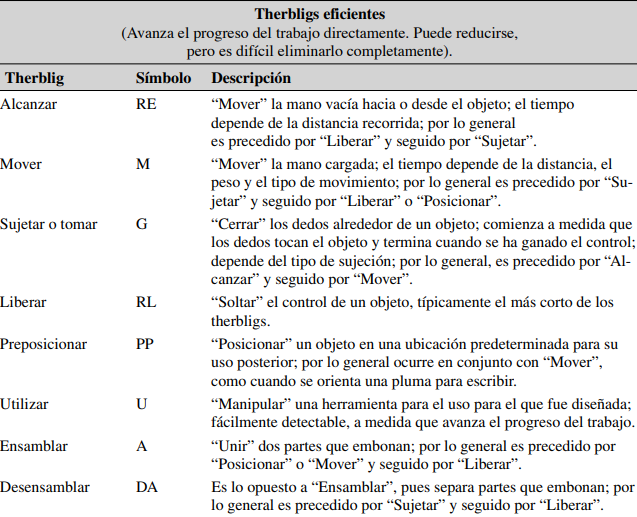
\includegraphics[scale=0.42]{35/Img/ther1.png}
        \caption{Therbligs Eficientes}
        \label{fig:therbligs1}
    \end{figure}
    % 
    
    % 
    \begin{figure}[H]
        \centering
        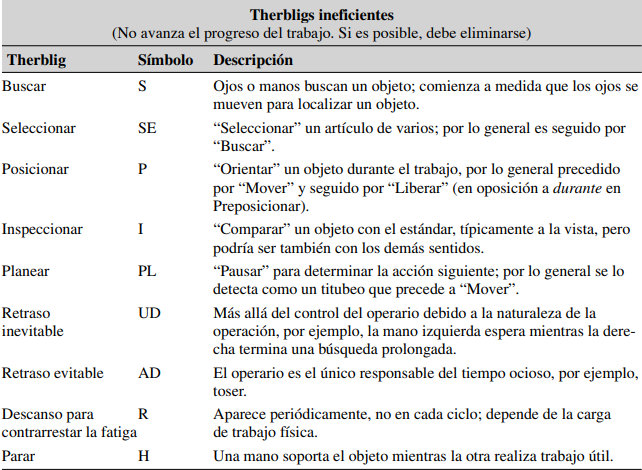
\includegraphics[scale=0.42]{35/Img/ther2.png}
        \caption{Therbligs Ineficientes}
        \label{fig:therbligs2}
    \end{figure}
    % 
    
    
    \section{Hipótesis}
    
    Realizar un proyecto integrador en cual se apliquen conocimientos adquiridos en la materia de Estudio del Trabajo y comprender a fondo como es el desarrollo de un proyecto de estudio de tiempos implementando distintos métodos como el muestreo, STP y tiempo estándar.
    
    
    \begin{itemize}
        \item Se debe de identificar claramente la suposición científica
        \item Se debe de identificar claramente el fundamento científico
        \item Se debe identificar claramente la variable de respuesta
        \item Se debe identifican claramente las realidades o modelos contrastantes
        \item Se debe de establecer las variables asociadas, explicativas o que tienen relación funcional con la variable de respuesta
    \end{itemize}
    % 
    % 
    \section{Objetivo}
    Diseñar y mejorar sistemas para aumentar la productividad del proyecto integrador del circuito electrónico aplicando todas las herramientas y técnicas que se ha adquirido en un plazo de un semestre escolar (4 meses aproximadamente).
    
    \subsection{Objetivos específicos }
    
    \begin{itemize}
        \item Analizar los métodos, materiales, herramientas e instalación utilizada o que se ha de utilizar en la ejecución del ensamble de un circuito electrónico.
        \item Buscar la manera mas económica de realizar el trabajo.
        \item Implementar un plan de emergencia de las instalaciones.
        \item Investigar y proponer mejoras en el diseño del circuito electrónico para facilitar su ensamble, reducir la complejidad y el número de pasos requeridos.
        \item Normalizar los métodos, materiales, herramientas e instalaciones.
        
    
    \end{itemize}
    
    % 
    % 
    \section{Metodología} %\ref{anexo:manual}.
    
    Este estudio de investigación se llevó a cabo utilizando métodos de observación y análisis estadístico. La recolección de datos y el análisis se realizaron en la ciudad de Querétaro, en las instalaciones del Instituto Tecnológico de Queretaro, durante el periodo comprendido entre febrero y mayo de 2024.
    
    Para el estudio se utilizo el armado de un circuito  conformado principalmente por una tarjeta ESP32-C6.
    En la primera etapa del experimento, se tomaron dos muestras continuas con una cámara de vídeo. Posteriormente, se aplicaron varias metodologías para determinar el tiempo de ciclo y el tiempo estándar.
    
    Antes de realizar el ensamble del circuito se debe de asegurar que todos los materiales estén completos y en un estado óptimo; Un punto importante en el proceso del proyecto integrador es el conocer a detalle cada uno de los materiales que se han de utilizar pues un conocimiento a fondo de todos los materiales se traduce en un mejor desempeño del operario y además es fundamental en la estandarización de las herramientas, materiales e instalaciones, por ello mismo se debe en listar cada parte del ensamblaje para que a la hora del desarrollo del estudio tengamos una secuencia con orden. Véase los materiales necesarios para el ensamble en la siguiente lista:
    % 
    \begin{figure}[H]
        \centering
        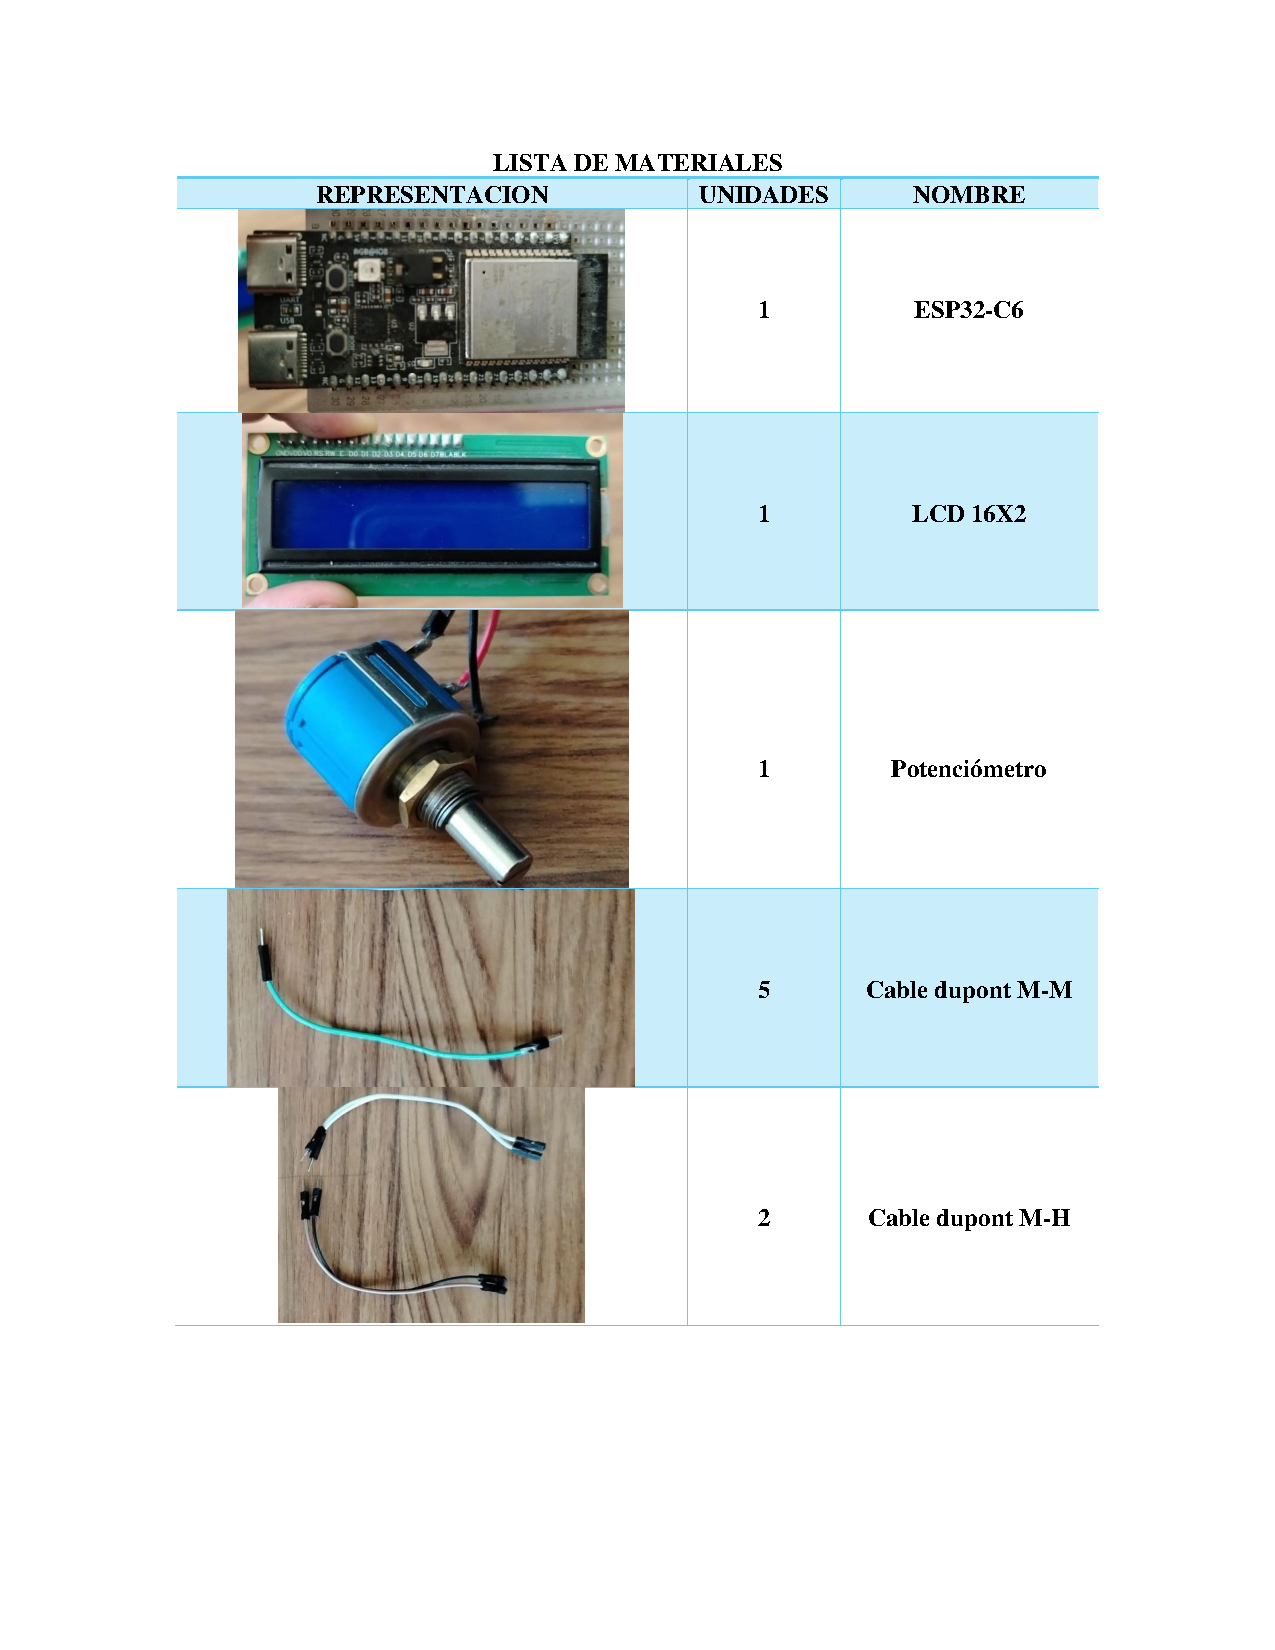
\includegraphics[scale=0.4]{35/Img/listaMateriales.pdf}
        \caption{lista deMateriales}
        \label{fig:listamateriales}
    \end{figure}
    % 
    La organización en la industria es crucial para optimizar los procesos y garantizar la eficiencia operativa. Una buena organización permite una mejor gestión del tiempo y los recursos, reduciendo costos y aumentando la productividad. En el ensamblaje de un circuito electrónico, un bosquejo de distribución de materiales es esencial. Este plan asegura que todos los componentes estén correctamente ubicados y accesibles, lo que minimiza errores y retrasos. Además, una distribución eficiente facilita el flujo de trabajo y mejora la calidad del producto final, contribuyendo a un proceso mas óptimo del trabajo. 
    % 
    \begin{figure}[H]
        \centering
        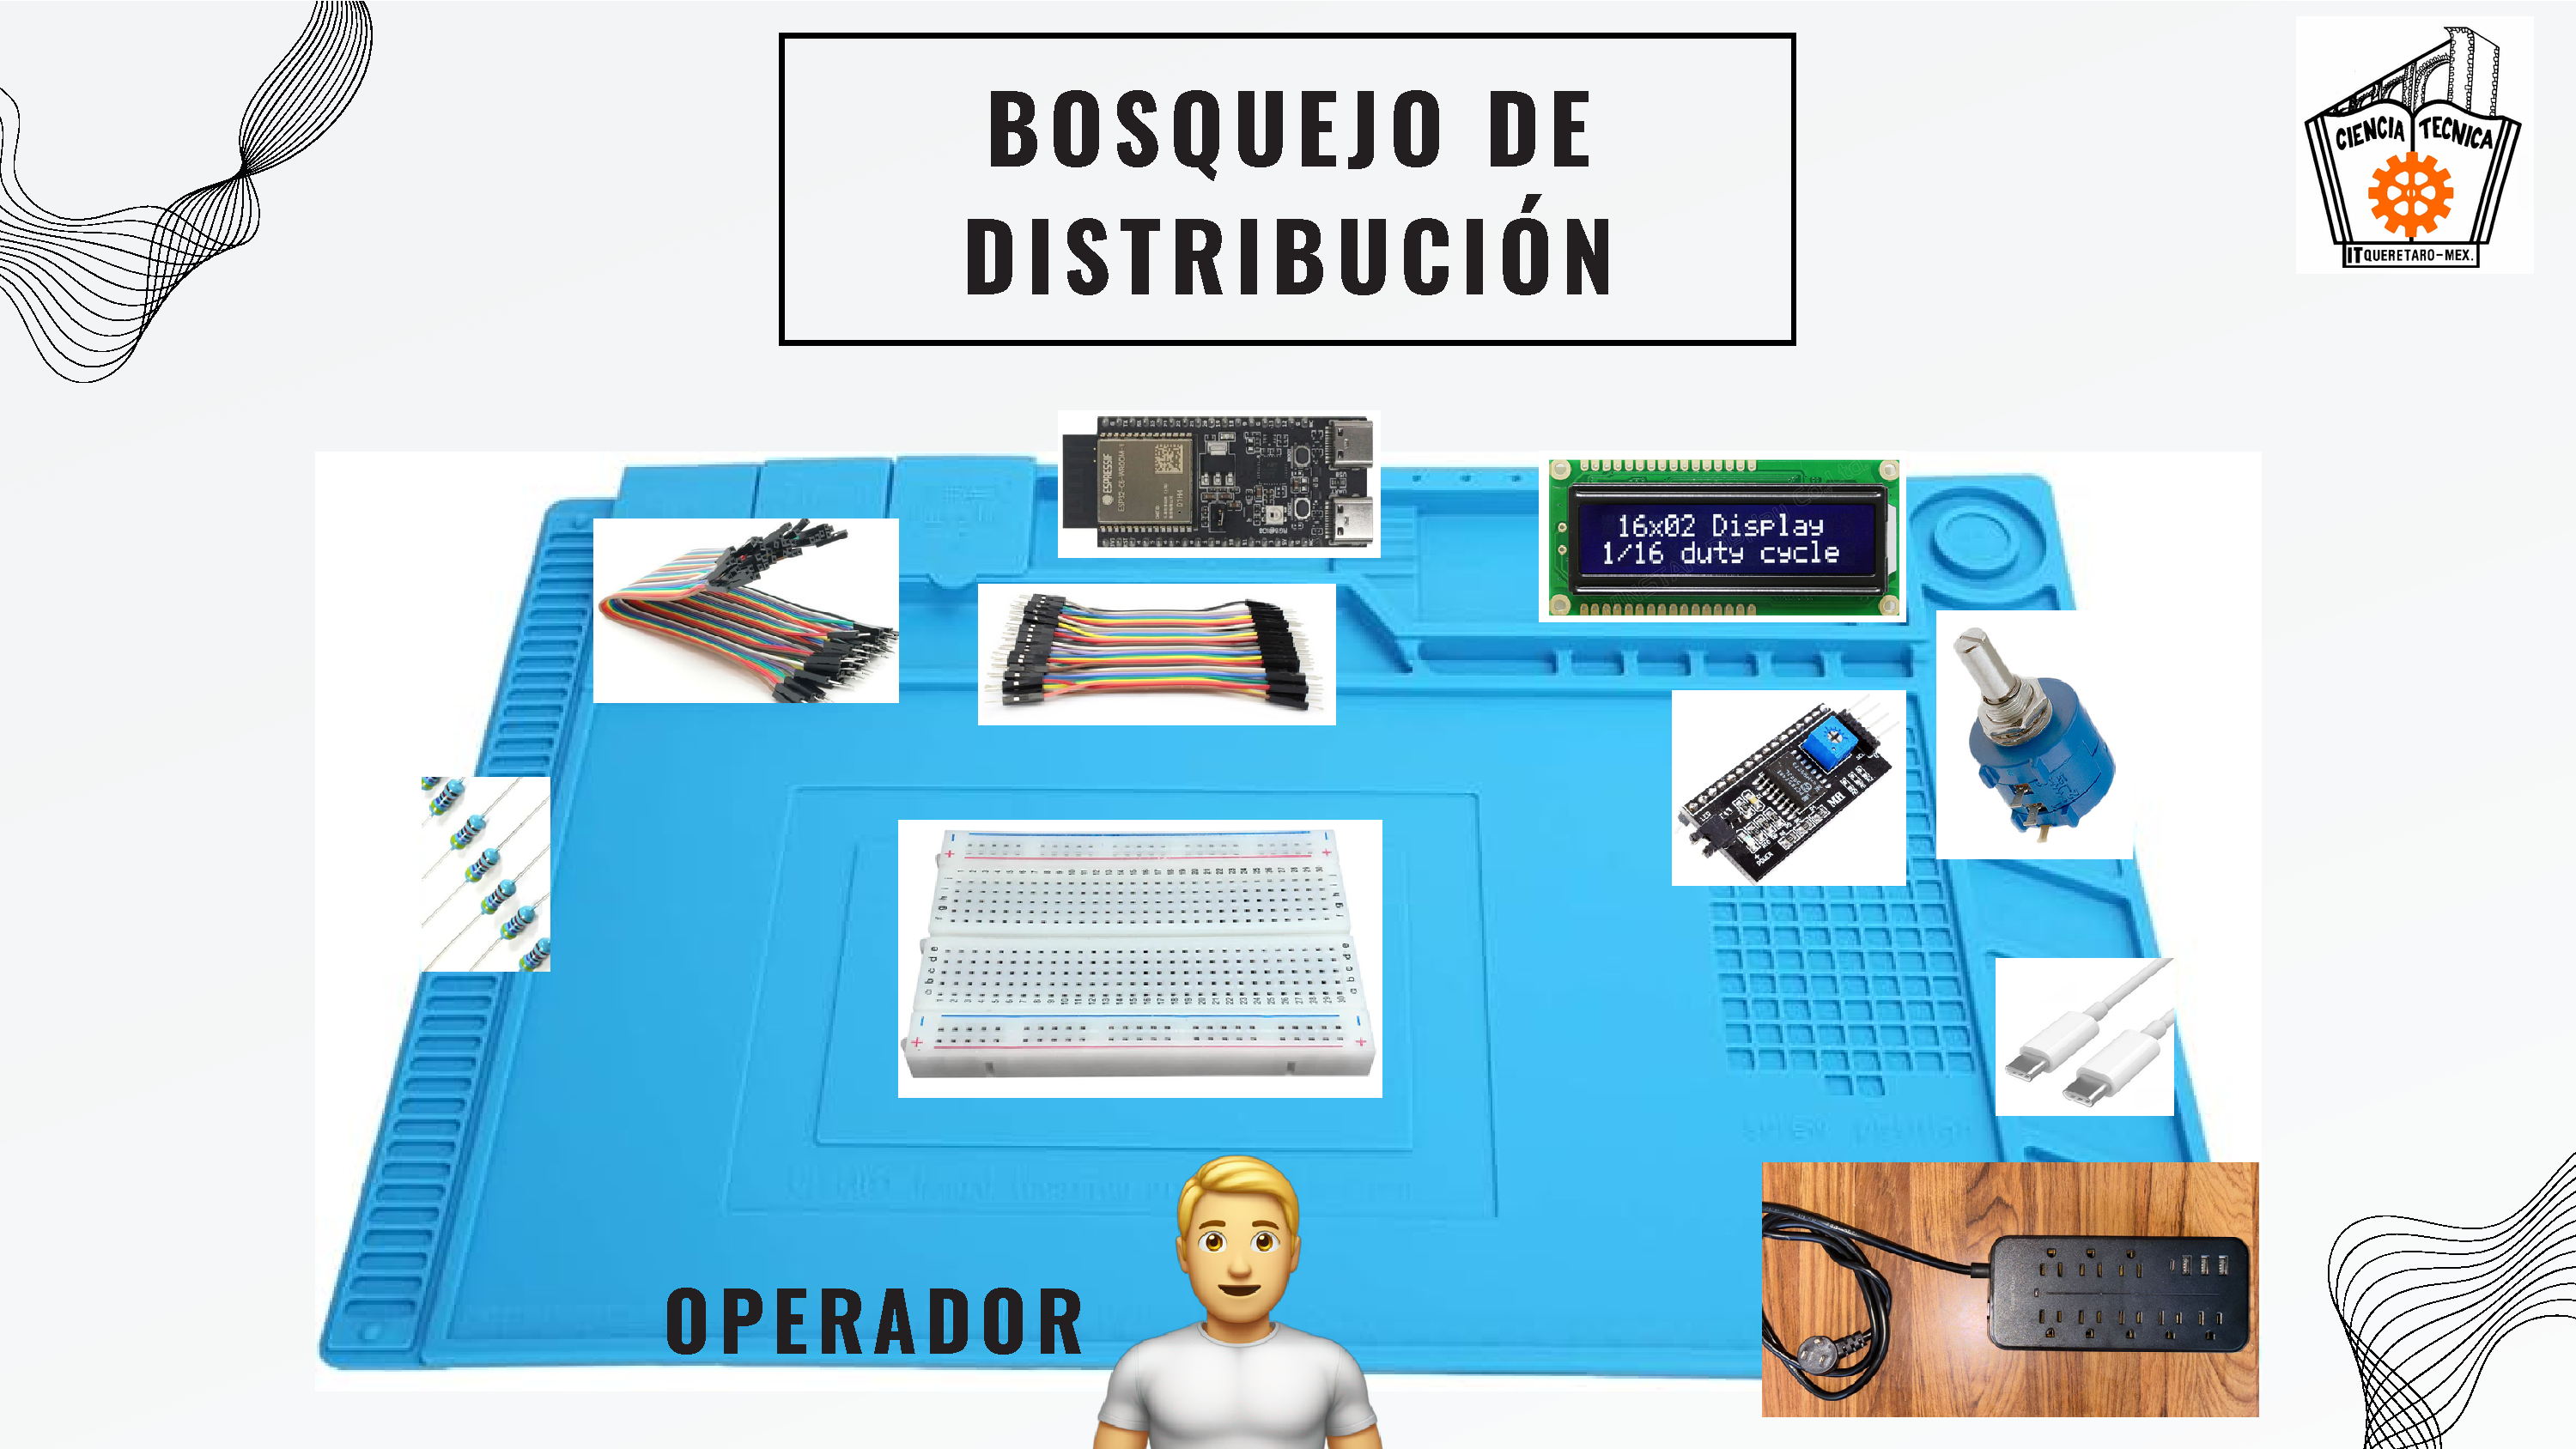
\includegraphics[scale=0.16]{35/Img/bosquejoDistribucion.pdf}
        \caption{Bosquejo de distribución}
        \label{fig:bosquejoDistribucion}
    \end{figure}
    % 
    
    
    La implementación de una ayuda visual, como un manual de pasos del proceso, es fundamental en la industria para garantizar la claridad y uniformidad en la ejecución de tareas. Este tipo de herramienta guía a los trabajadores, reduciendo el riesgo de errores y aumentando la eficiencia. En el caso de un proyecto integrador, como el ensamblaje de un circuito electrónico, un manual detallado es crucial. Proporciona instrucciones precisas para cada etapa del ensamblaje, asegurando que todos los componentes se coloquen correctamente y en el orden adecuado. Esto no solo mejora la calidad del producto final, sino que también facilita la formación y adaptación de nuevos operadores al proceso.
    Véase el manual de ensamble en el siguiente documento \ref{anexo:manual}.
    
    \subsection{Desarrollo de la guía de plan de Emergencia}
    
    Documento que describe los lineamientos a seguir, la organización y los mecanismos, que indican la manera de enfrentar una situación de emergencia. Cuyo objetivo es implementar las estrategias para proporcionar seguridad a las personas, sus bienes y todo lo que rodea mediante procedimientos antes, durante y después de una situación de emergencia.
    
    \subsection{Análisis de los métodos, materiales, herramientas e instalación utilizada en la ejecución del ensamble de un circuito electrónico}
    
    \subsubsection{Planeación}
    
    Asegúrate de conocer siempre tu objetivo.
    Asegúrate de contar con los documentos (formatos, procedimientos, etc).
    % 
    % 
    \subsubsection{5's}
    
    Las 5´s son un programa de trabajo que consiste en desarrollar actividades de orden/limpieza y detección de anomalías en el puesto de trabajo, que por su sencillez permiten la participación de todos a nivel individual/grupal, mejorando el ambiente de trabajo, la seguridad de personas y equipos y la productividad.
    
    En el proyecto integrador se aplicaron de la siguiente manera:
    
    \begin{itemize}
        \item Seiri (Clasificación)
    \end{itemize}
    
    - Identificación Materiales: Realizar una lista de todos y materiales utilizados en el proceso de ensamblaje.
    \newline
    - Frecuencia de Uso: Clasificar los materiales restantes según su frecuencia de uso, asegurando que los más utilizados estén más accesibles.
    
    \begin{itemize}
        \item Seiton (Orden)
    \end{itemize}
    - Diseño del Área de Trabajo: Crear un diseño lógico del área de trabajo donde cada material tenga un lugar designado; se implemento mediante un bosquejo de distribución.
    
    \begin{itemize}
        \item Seiso (Limpieza)
    \end{itemize}
    -Mantener espacio limpio: Limpiar el espacio de trabajo antes y después de realizar el trabajo.
    \newline
    -Inspección y Mantenimiento: Realizar inspecciones regulares para asegurar que el equipo este en buen estado y funcionando correctamente.
    
    \begin{itemize}
        \item Seiketsu (Estandarización)
    \end{itemize}
    
    -Procedimientos Estándar: Crear procedimientos estándar para las tareas diarias de limpieza y organización.
    \newline
    -Documentación: Documentar los procedimientos y asegurarse de que estén disponibles para todos los miembros del equipo.
    
    \begin{itemize}
        \item Shitsuke (Disciplina)
    \end{itemize}
    
    -Retroalimentación Continua: Proporcionar retroalimentación continua y reconocer el buen desempeño en la implementación de las 5S.
    
    
    %https://books.google.com.mx/books?hl=es&lr=&id=NJtWepnesqAC&oi=fnd&pg=PA13&dq=5S&ots=8vv9fhoWbB&sig=_ZRz2WT14l3Y6PXMCfwc6aIIU1Y#v=onepage&q&f=false
    
    \subsubsection{Desarrollo del sistema de tiempos predeterminado}
    % 
    % 
    \subsubsection{Desarrollo del muestreo del trabajo}
    El muestreo del trabajo es una técnica que se utiliza para investigar las proporciones del tiempo total que se dedican a las diferentes actividades que constituyen una tarea o una situación de trabajo. Los resultados del muestreo del trabajo son eficaces para determinar la utilización de máquinas y personal, las holguras aplicables al trabajo y los estándares de producción. Aunque se puede obtener la misma información con procedimientos de estudio de tiempos, el muestreo del trabajo con frecuencia proporciona estos datos más rápido y a un costo considerablemente menor.
    %libro nievel
    % 
    \subsubsection{Corrección por balanceo de procesos}
    % 
    % 
    \subsubsection{Datos estándar continuos y discretos}
    Los datos estándar permiten el rápido establecimiento de tiempos estándar precisos antes de que se realice el trabajo. Esta característica hace que su uso sea especialmente atractivo para estimar el costo de un nuevo trabajo, con propósitos de presupuesto y subcontratación. La utilización de datos estándar también simplifica muchos problemas administrativos en las plantas donde puede haber restricciones concernientes a aspectos como el tipo de estudio que se llevará a cabo, el número de ciclos que se deben estudiar, los operarios que serán estudiados y el observador que realizará el estudio.
    
    \subsection{Diseño de la forma más económica de realizar el trabajo}
    
    % 
    % 
    \subsection{Normalización de los métodos, materiales, herramientas e instalaciones}
    
    % 
    % 
    \subsection{Determinación del tiempo estándar para que una persona competente realice el trabajo con marcha normal}
    
    
    \section{Resultados y discusión}
    
    \subsection{Desarrollo de la guía de plan de Emergencia}
    
    Esta guía ha sido creada con el objetivo de establecer un entorno seguro y libre de emergencias y accidentes en el Instituto Tecnológico de Querétaro. Nos dedicamos a identificar al personal que haya recibido formación especializada al menos una vez al año, asegurándonos de que estén bien preparados para enfrentar cualquier situación crítica. La capacitación continua del personal es fundamental para garantizar que, en caso de una emergencia, se adopten las mejores prácticas y se tomen decisiones rápidas y efectivas. Nuestro compromiso es proteger la integridad física de todos los que forman parte de la comunidad del instituto, incluidos estudiantes, profesores, empleados y visitantes, así como preservar las instalaciones para asegurar la continuidad de las actividades académicas y administrativas en un entorno seguro y protegido.
    Los datos generales del establecimiento son los siguientes:
    
    Tecnológico Nacional de México Campus Querétaro Plantel Centro
    Institución de educación superior y posgrado
    Superficie 82,456.01 metros cuadrados 
    Teléfono De contacto(442) 227 44 00
    Director: Ramón Soto Arriola
    Horario de Lunes a Viernes de 7:00 a 22:00 hrs.
    Alumnos Matriculados en 2022: 5,827 de los cuales 62.5 por ciento (3.66k) son hombres y 37.1 por ciento (2.16k) son mujeres.
    
    % 
    % 
    \begin{figure}[H]
        \centering
        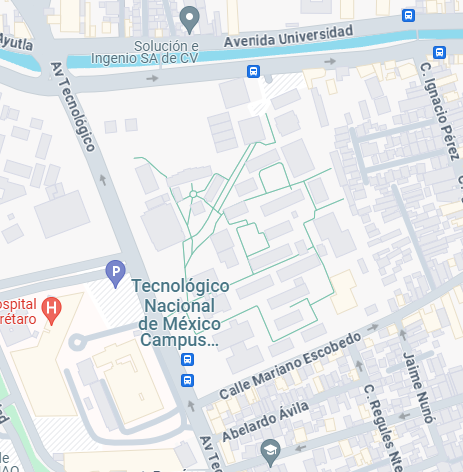
\includegraphics[scale=0.4]{35/Img/mapaITQ.png}
        \caption{Tecnológico Nacional de México, Instituto Tecnológico de Querétaro, Av Tecnológico S/N, Centro Histórico, Centro, 76000, Querétaro, Qro.}
        \label{fig:mapaITQ}
    \end{figure}
    % 
    % 
    
    \subsubsection{Identificación del riesgo}
    
    Estamos comprometidos a mantener un programa interno de prevención de riesgos todos los días. Este programa no solo se enfoca en la identificación y mitigación de posibles peligros, sino que también fomenta la retroalimentación constante del personal y de los alumnos. Valoramos enormemente sus observaciones sobre los riesgos que puedan surgir en el desarrollo de sus actividades diarias. Por ello, los animamos a utilizar el equipo de trabajo y a comunicar cualquier situación de riesgo que detecten.
    
    Cada riesgo interno que identificamos es evaluado según una escala de prioridad. Esta evaluación nos permite determinar cuáles acciones deben ser implementadas primero para garantizar la seguridad de todos.  
    
    % 
    \begin{figure}[H]
        \centering
        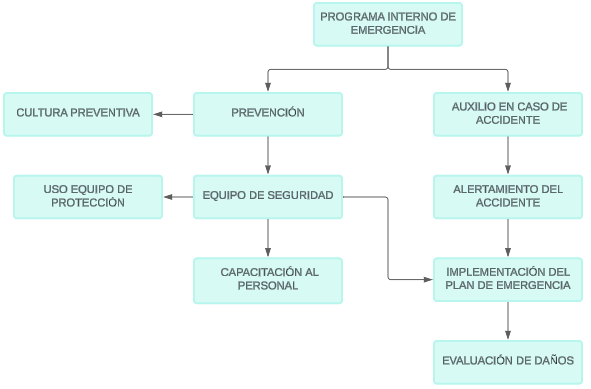
\includegraphics[scale=0.4]{35/Img/diagramaPE.png}
        \caption{Diagrama para la identificación de riesgos y acciones}
        % \label{fig:diagramaPE}
    \end{figure}
    % 
    
    \subsubsection{Riesgos internos}
    
    % 
    \begin{figure}[H]
        \centering
        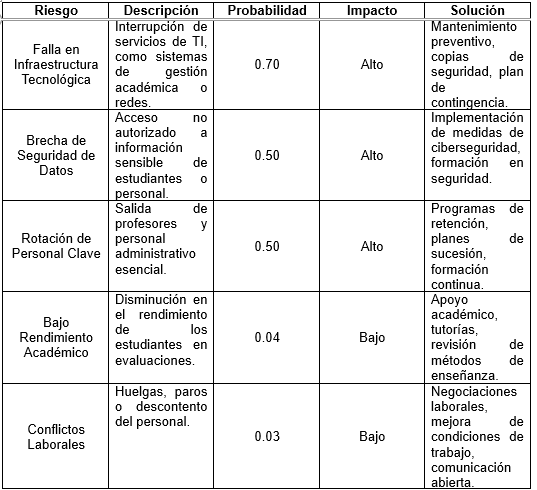
\includegraphics[scale=0.5]{35/Img/riesgosInternos.png}
        \caption{Descripción de los riesgos internos.}
        % \label{fig:riesgosInternos}
    \end{figure}
    % 
    
    \subsubsection{Riesgos externos}
    
    % 
    \begin{figure}[H]
        \centering
        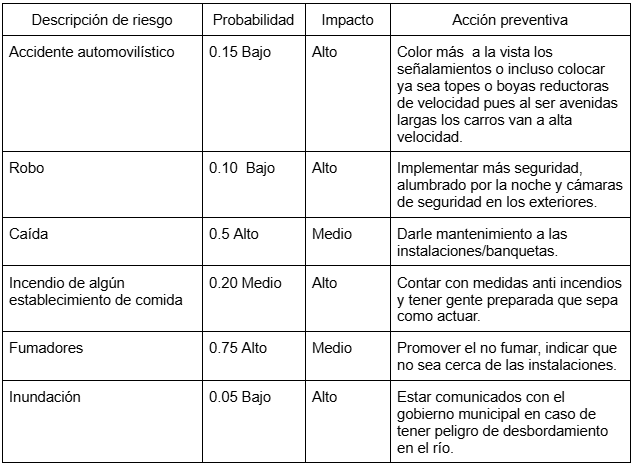
\includegraphics[scale=0.5]{35/Img/riesgosExternos.png}
        \caption{Descripción de los riesgos externos.}
        % \label{fig:riesgosEternos}
    \end{figure}
    % 
    
    \subsubsection{Programa de actividades de prevención y auxilio}
    
    Vamos a implementar un plan de prevención basado en los siguientes puntos:
    
    \begin{itemize}
        \item Ergonomía:Mejora de las estaciones de trabajo para reducir la fatiga y prevenir lesiones.
    \end{itemize}
    
    \begin{itemize}
        \item Capacitación: Entrenamiento continuo en técnicas de trabajo seguro y eficiente, además de cursos de primeros auxilios y participar e implementar en simulacros en caso de desastre.
    \end{itemize}
    \begin{itemize}
        \item Equipos de Protección: Uso obligatorio del equipo de protección adecuado.
    \end{itemize}
    \begin{itemize}
        \item Monitorio Continuo: Sistema de monitorio continuo para identificar y corregir rápidamente cualquier problema.
    \end{itemize}
    
    \subsubsection{Plan de acción}
    
    \subsubsection{Identificación de capacidades}
    
    \begin{figure}[H]
        \centering
        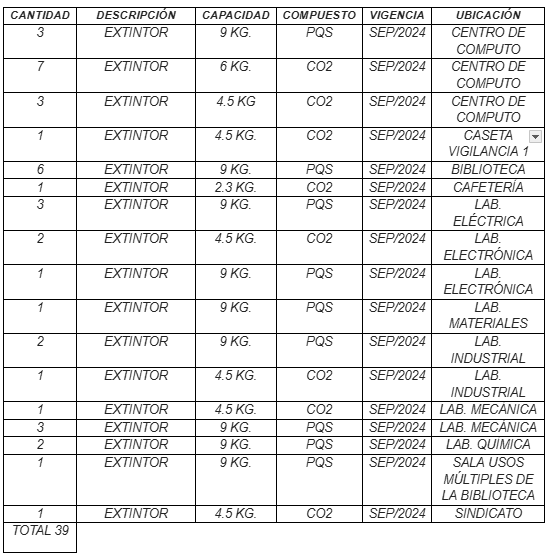
\includegraphics[scale=0.5]{35/Img/extintores.png}
        \caption{Recursos en materia de extintores.}
        % \label{fig:extintores}
    \end{figure}
    % 
    
    \subsubsection{Plano de localización de recursos}
    \begin{figure}[H]
        \centering
        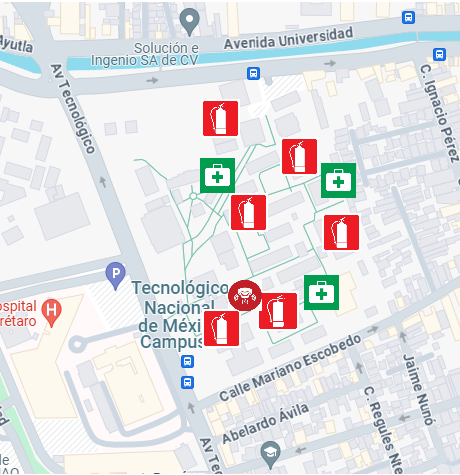
\includegraphics[scale=0.45]{35/Img/mapaEB.png}
        \caption{Plano del establecimiento de los recursos en materia de seguridad.}
        % \label{fig:mapaEB}
    \end{figure}
    % 
    
    \subsubsection{ Identificación de apoyos externos}
    
    \begin{figure}[H]
        \centering
        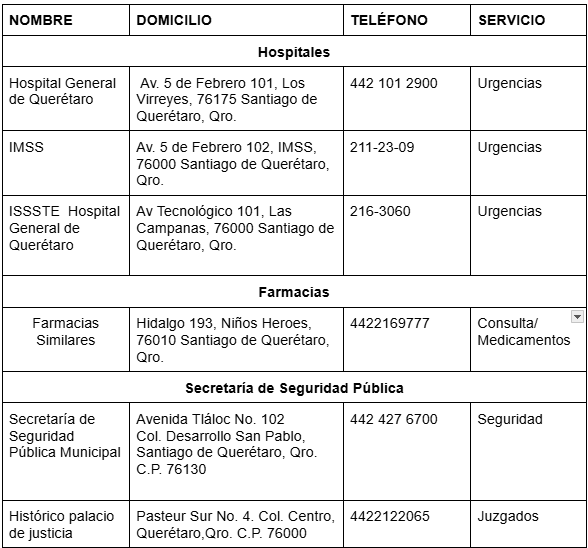
\includegraphics[scale=0.5]{35/Img/apoyosExternos.png}
        \caption{Lugares que servirán de apoyo en un situación de emergencia.}
        % \label{fig:apoyosExternos}
    \end{figure}
    % 
    
    \subsubsection{Identificación de puntos de reunión}
    
    % 
    \begin{figure}[H]
        \centering
        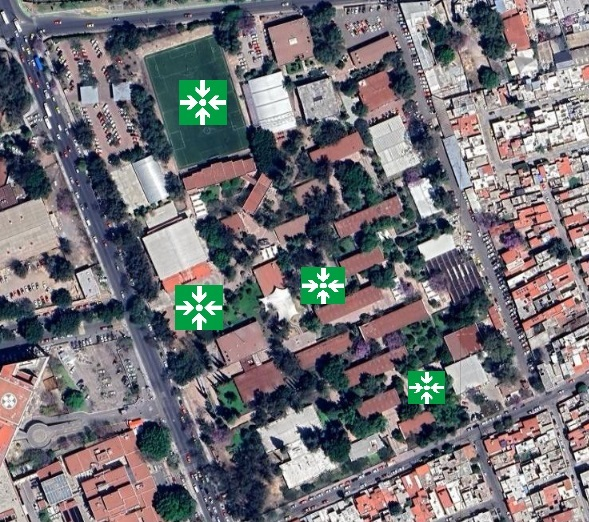
\includegraphics[scale=0.4]{35/Img/puntosReunion.jpg}
        \caption{Zona segura en caso de una evacuación de emergencia.}
        % \label{fig:my_label}
    \end{figure}
    % 
    
    \subsubsection{Brigada de evacuación}
    
    Una brigada de evacuación en el tecnológico es fundamental para garantizar la seguridad y el bienestar de estudiantes, profesores y personal administrativo en situaciones de emergencia. Estas brigadas están entrenadas para coordinar y guiar la evacuación ordenada y eficiente de los edificios en casos de incendios, terremotos u otras emergencias, minimizando el riesgo de lesiones y pánico. Su presencia y preparación son cruciales para asegurar que todos los ocupantes conozcan las rutas de escape y los procedimientos adecuados, contribuyendo a una respuesta rápida y efectiva que puede salvar vidas. Véase la con detalle las 3 fases de la brigada en el documento
    % 
    \begin{figure}[H]
        \centering
        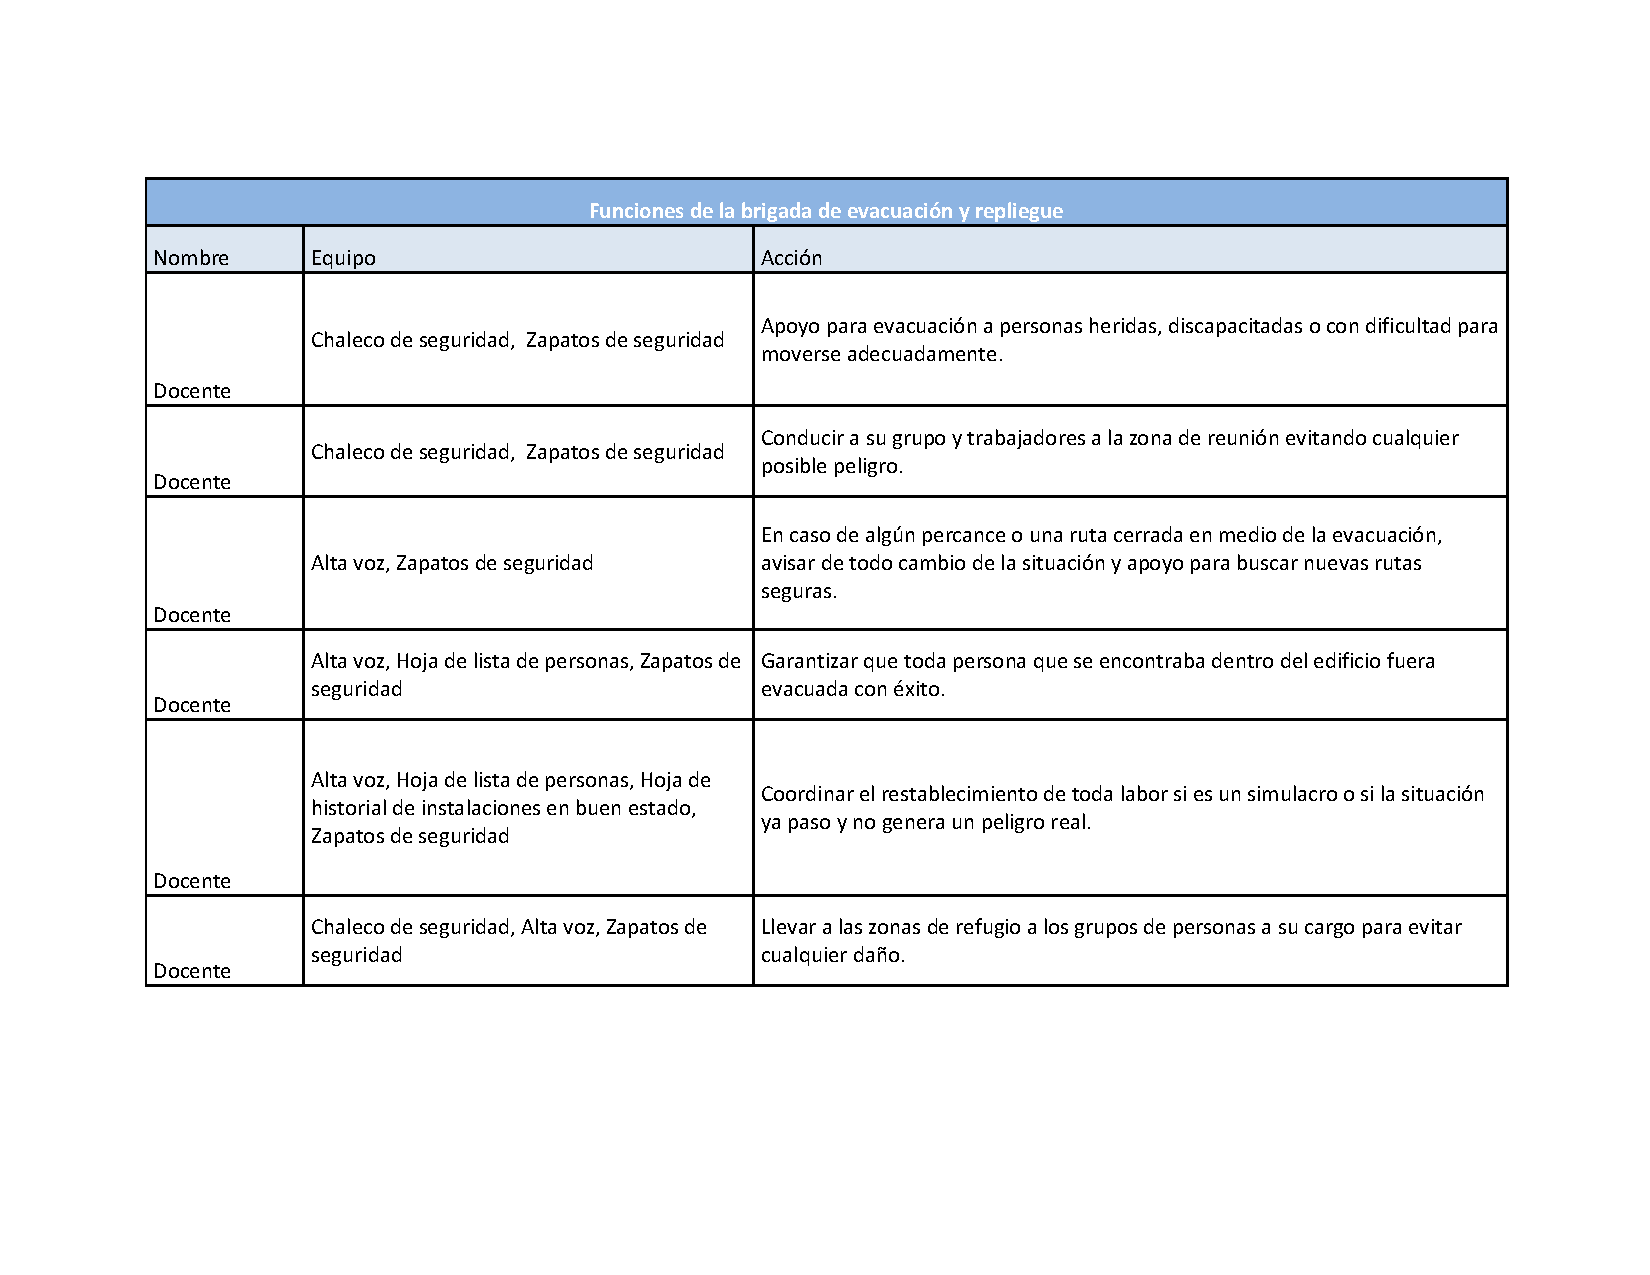
\includegraphics[scale=0.13]{35/Img/brigadaEvacuacion.pdf}
        \caption{Zona segura en caso de una evacuación de emergencia.}
        % \label{fig:my_label}
    \end{figure}
    
    
    \subsubsection{Directorio de telefónicos de emergencia}
    
    % 
    \begin{figure}[H]
        \centering
        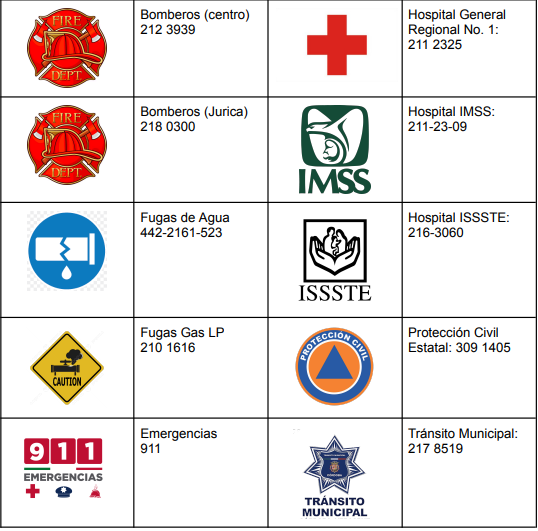
\includegraphics[scale=0.5]{35/Img/directorio.png}
        \caption{Listado telefónico de instituciones de atención de emergencias y otras instituciones que intervengan para el seguimiento y control de las mismas.}
        % \label{fig:my_label}
    \end{figure}
    % 
    
    \subsection{Análisis de los métodos, materiales, herramientas e instalación utilizada en la ejecución del ensamble de un circuito electrónico}
    
    \subsubsection{Verificación}
    
    Costos de no calidad.
    % 
    % 
    \subsubsection{Desarrollo del sistema de tiempos predeterminado}
    
    Para el desarrollo del sistema de tiempos predeterminados necesitamos dividir en partes o en actividades nuestro ensamble, para ellos se elaboro un diagrama bimanual de todo el proceso del ensamble. Este diagrama se divide en cada una de las actividades y describe con exactitud como se llevo a cabo el proceso, pues se indica en que secuencias se llevaron a cabo e indica con que mano se realizo cada acción.
    
    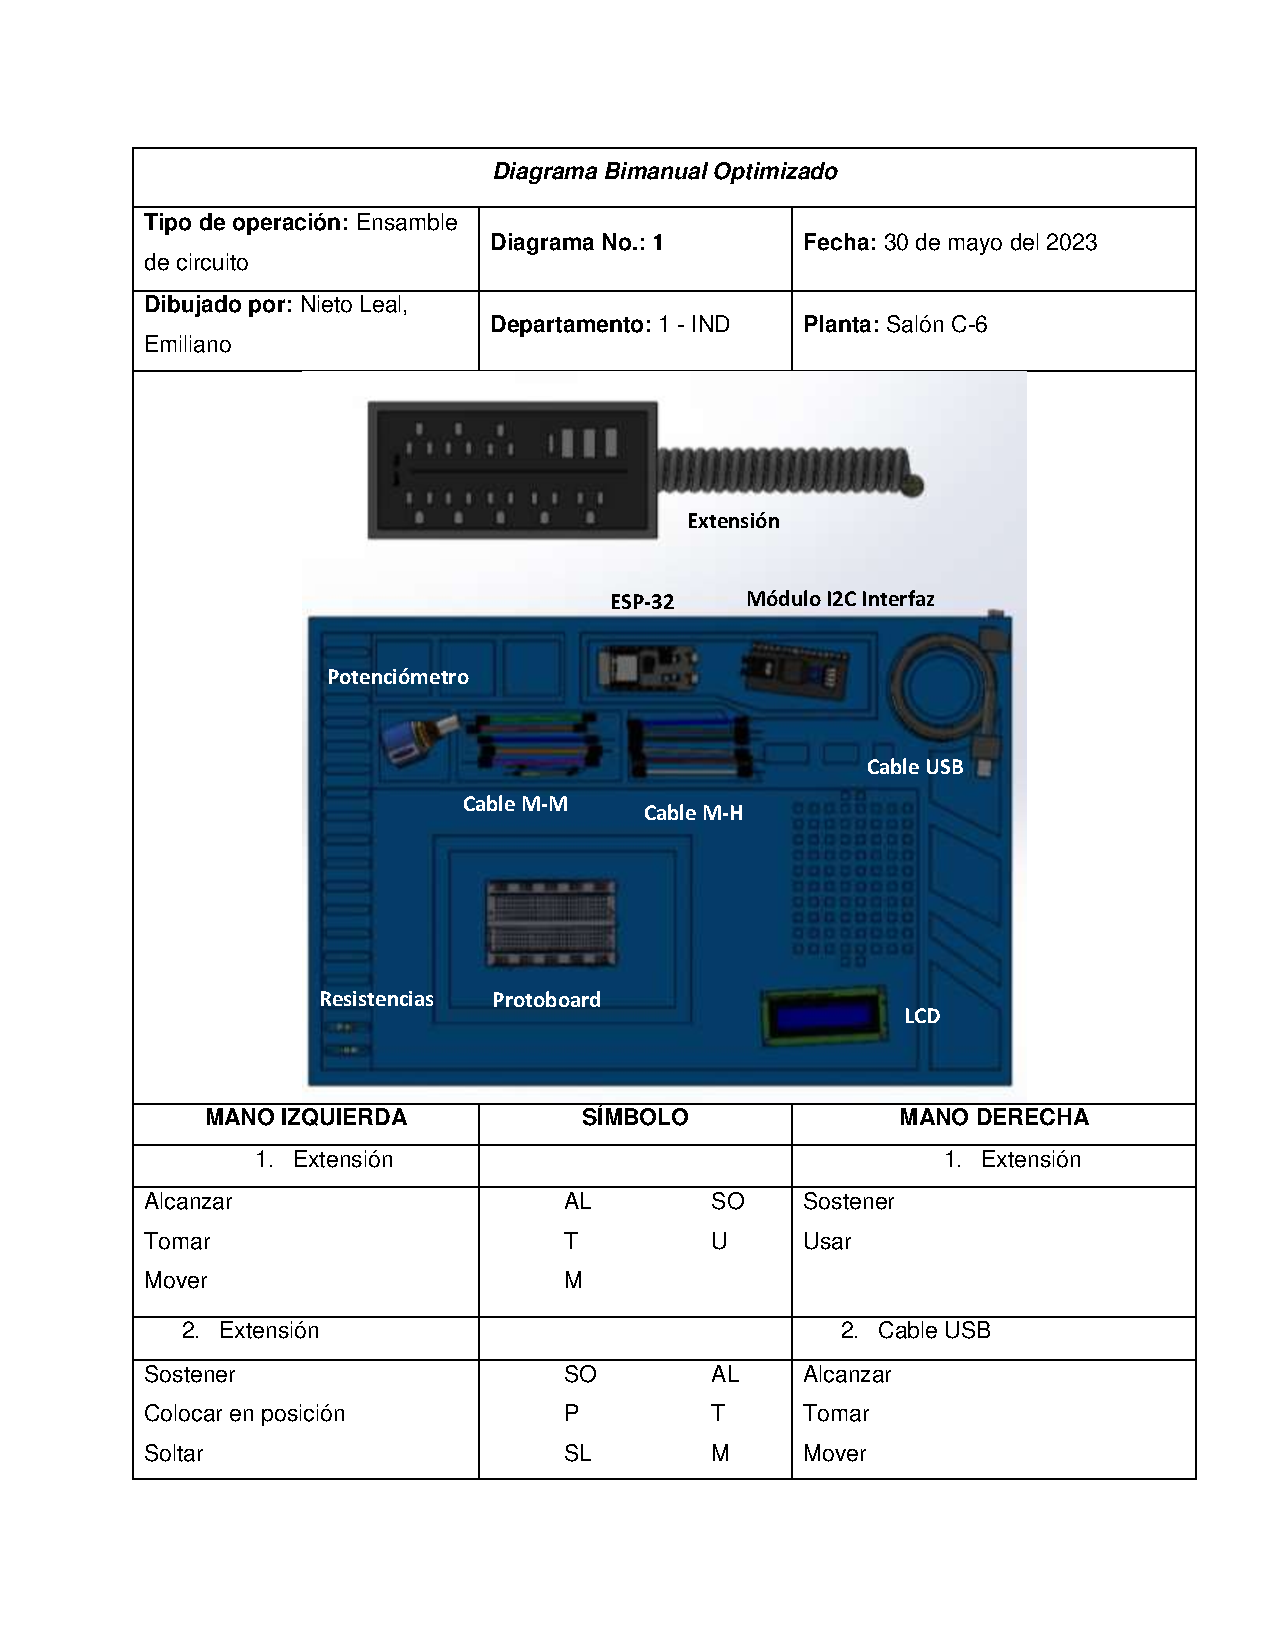
\includepdf[pages=-]{35/Img/diagramaBimanual.pdf}
    
    
     
     
    \subsubsection{Desarrollo del muestreo del trabajo}
    Para determinar el tiempo de ciclo, se desarrolló un método de muestreo que emplea un enfoque probabilístico. Para ello, se tomaron dos muestras en diferentes momentos, ya que son variables mutuamente excluyentes. Nuestro objetivo es encontrar una muestra que describa con precisión nuestro valor real.
    
    Los datos de la toma de la 1ra muestra son los siguientes:
    \newline
    Muestra 1
    \newline
    Operador: Nancy Ruiz Peña
    \newline
    Fecha: Miércoles 8 de Mayo del 2024
    \newline
    Hora de inicio: 4:53pm
    \newline
    Lugar: Instalaciones Instituto Tecnológico de Queretaro
    \newline
    Planta: Pasillo edificio F
    \newline
    Duración: 2:58 minutos
    \newline
    ´
    \begin{figure}[H]
        \centering
        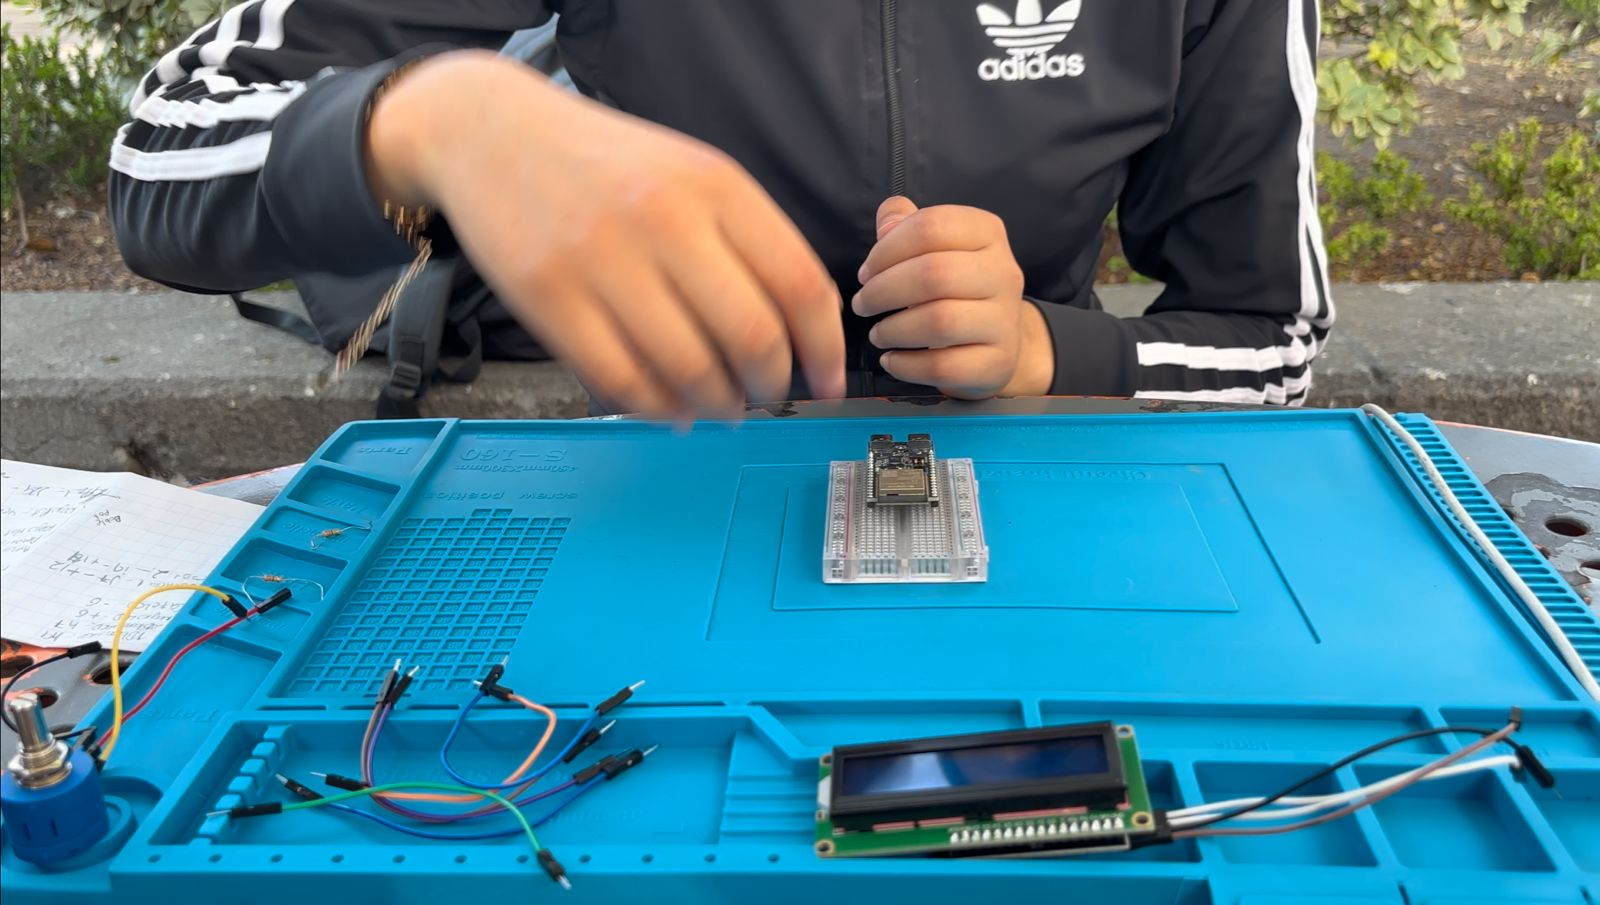
\includegraphics[scale=0.15]{35/Img/evidenciaM11.jpeg}
        \caption{Inicio del ensamble}
        % \label{Incio M1}
    \end{figure}
    
    \begin{figure}[H]
        \centering
        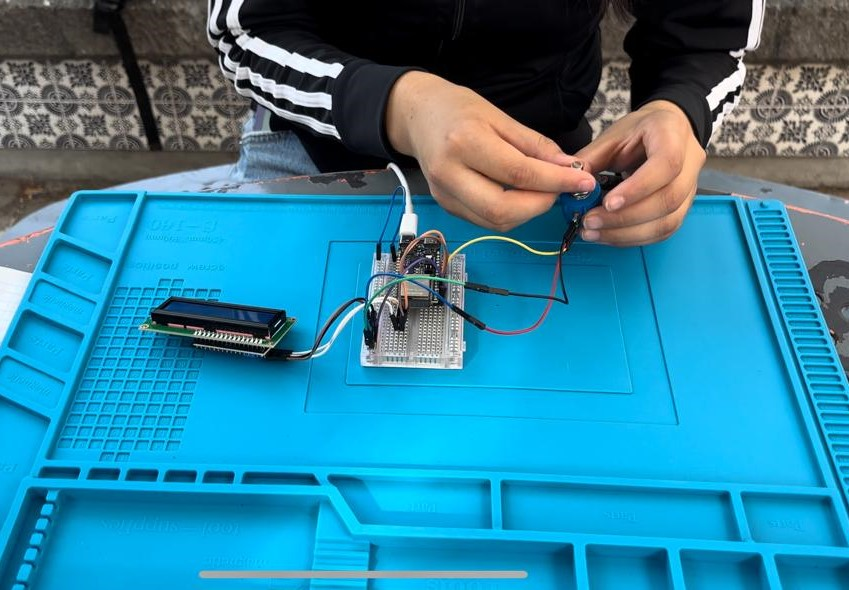
\includegraphics[scale=0.34]{35/Img/evidenciaM12.jpeg}
        \caption{Interacción con el potenciómetro}
        % \label{EM12}
    \end{figure}
    
    
    \begin{figure}[H]
        \centering
        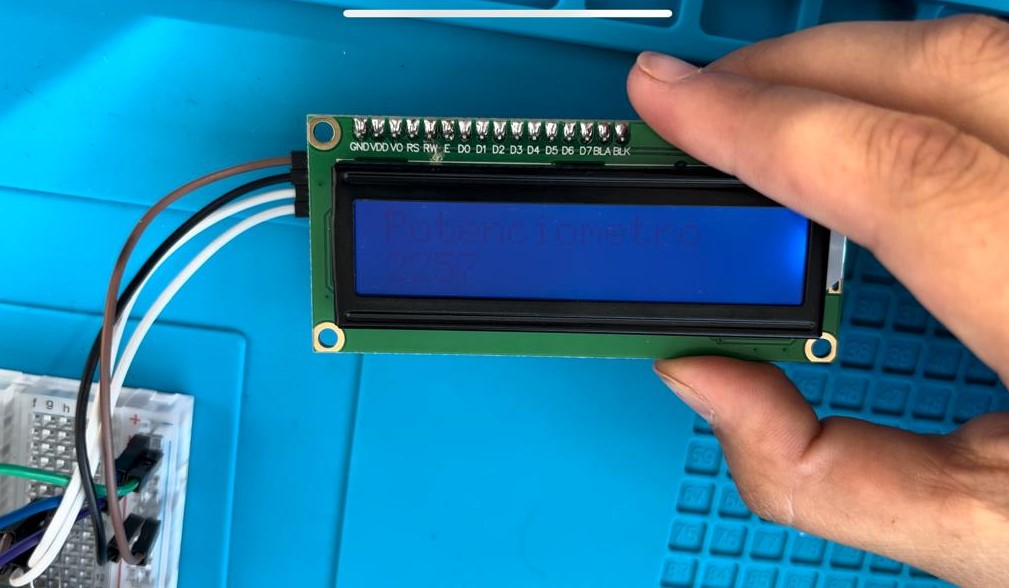
\includegraphics[scale=0.28]{35/Img/evidenciaM13.jpeg}
        \caption{Lectura del LCD}
        % \label{EM13}
    \end{figure}
    
    Los datos de la toma de la 2da muestra son los siguientes:
    \newline
    Muestra 1
    \newline
    Operador: Nancy Ruiz Peña
    \newline
    Fecha: Jueves 9 de Mayo del 2024
    \newline
    Hora de inicio: 4:50pm
    \newline
    Lugar: Instalaciones Instituto Tecnológico de Queretaro
    \newline
    Planta: Pasillo edificio F
    \newline
    Duración: 3:21 minutos
    \newline
    
    
    \begin{figure}[H]
        \centering
        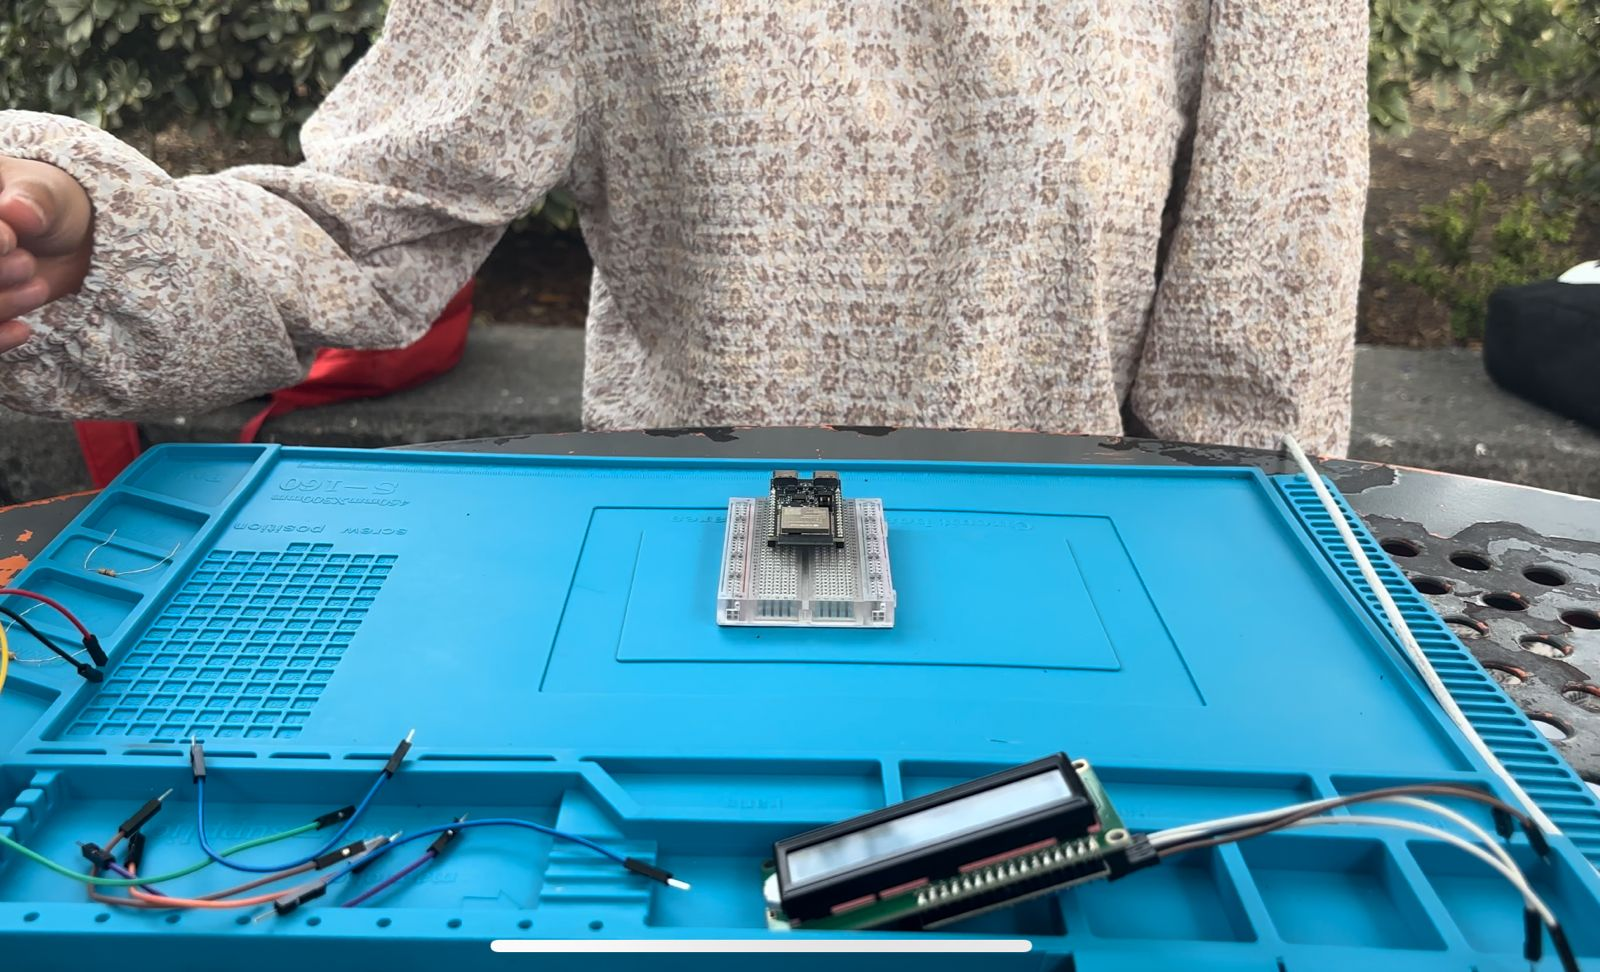
\includegraphics[scale=0.15]{35/Img/evidenciaM21.jpeg}
        \caption{Inicio del ensamble}
        % \label{Incio M1}
    \end{figure}
    
    \begin{figure}[H]
        \centering
        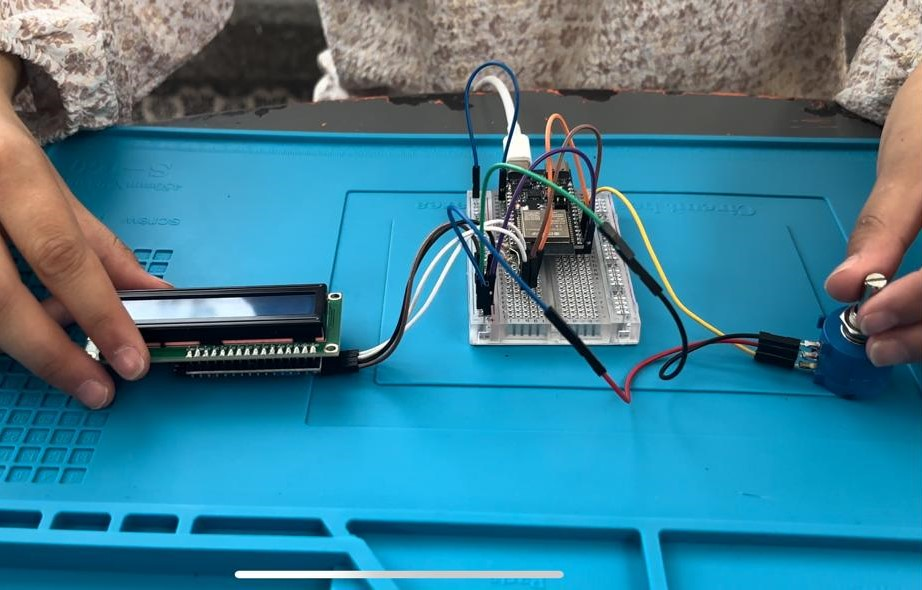
\includegraphics[scale=0.34]{35/Img/evidenciaM22.jpeg}
        \caption{Interacción con el potenciómetro}
        % \label{EM12}
    \end{figure}
    
    
    \begin{figure}[H]
        \centering
        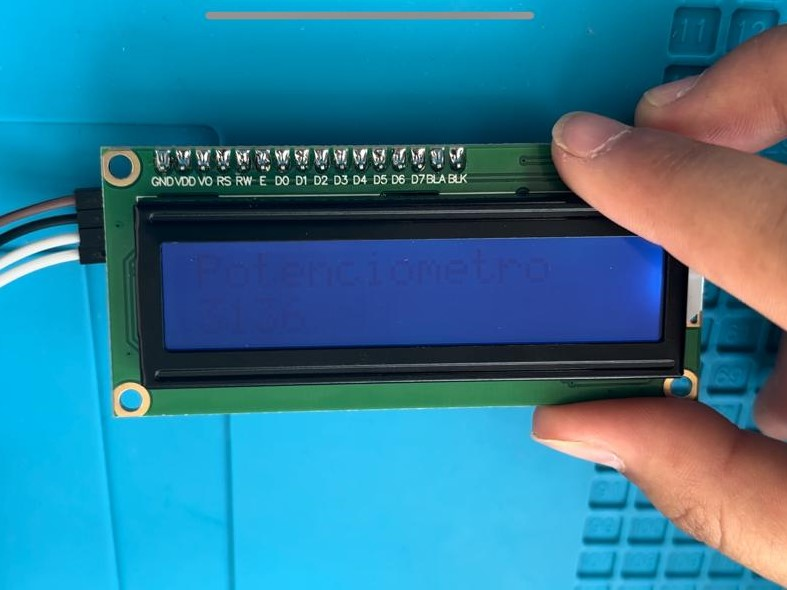
\includegraphics[scale=0.28]{35/Img/evidenciaM23.jpeg}
        \caption{Lectura del LCD}
        % \label{EM13}
    \end{figure}
    
    
    
    Con estas muestras tomadas, procederemos a calcular tanto el tiempo de ciclo como el tiempo estándar. Para esto, nos guiaremos en una película (un vídeo) que actúa como una muestra continua. A partir de este vídeo, se creó una hoja de datos en Excel para determinar el tiempo de ciclo de cada elemento individualmente. Nuestro trabajo se dividió en 12 elementos, por lo que tenemos 12 tiempos de ciclo individuales. Estos tiempos se promediaron a partir del tiempo en minutos que el operador tardó en las dos muestras. Para determinar esto, se observaron los dos vídeos recopilados, identificando los puntos de quiebre entre cada actividad para calcular el tiempo de cada elemento.
    
    
    % 
    % 
    \subsubsection{Corrección por balanceo de procesos}
    % 
    % 
    \subsubsection{Datos estándar continuos y discretos}
    % 
    % 
    \subsection{Diseño de la forma más económica de realizar el trabajo}
    
    % 
    % 
    \subsection{Normalización de los métodos, materiales, herramientas e instalaciones}
    
    % 
    % 
    \subsection{Determinación del tiempo estándar para que una persona competente realice el trabajo con marcha normal}
    
    Se obtuvo el tiempo ciclo de todas las actividades de las 2 muestras tomadas con los siguientes resultados: 
    \newline
    Tiempo de ciclo total: 3.15 minutos / 189 segundos
    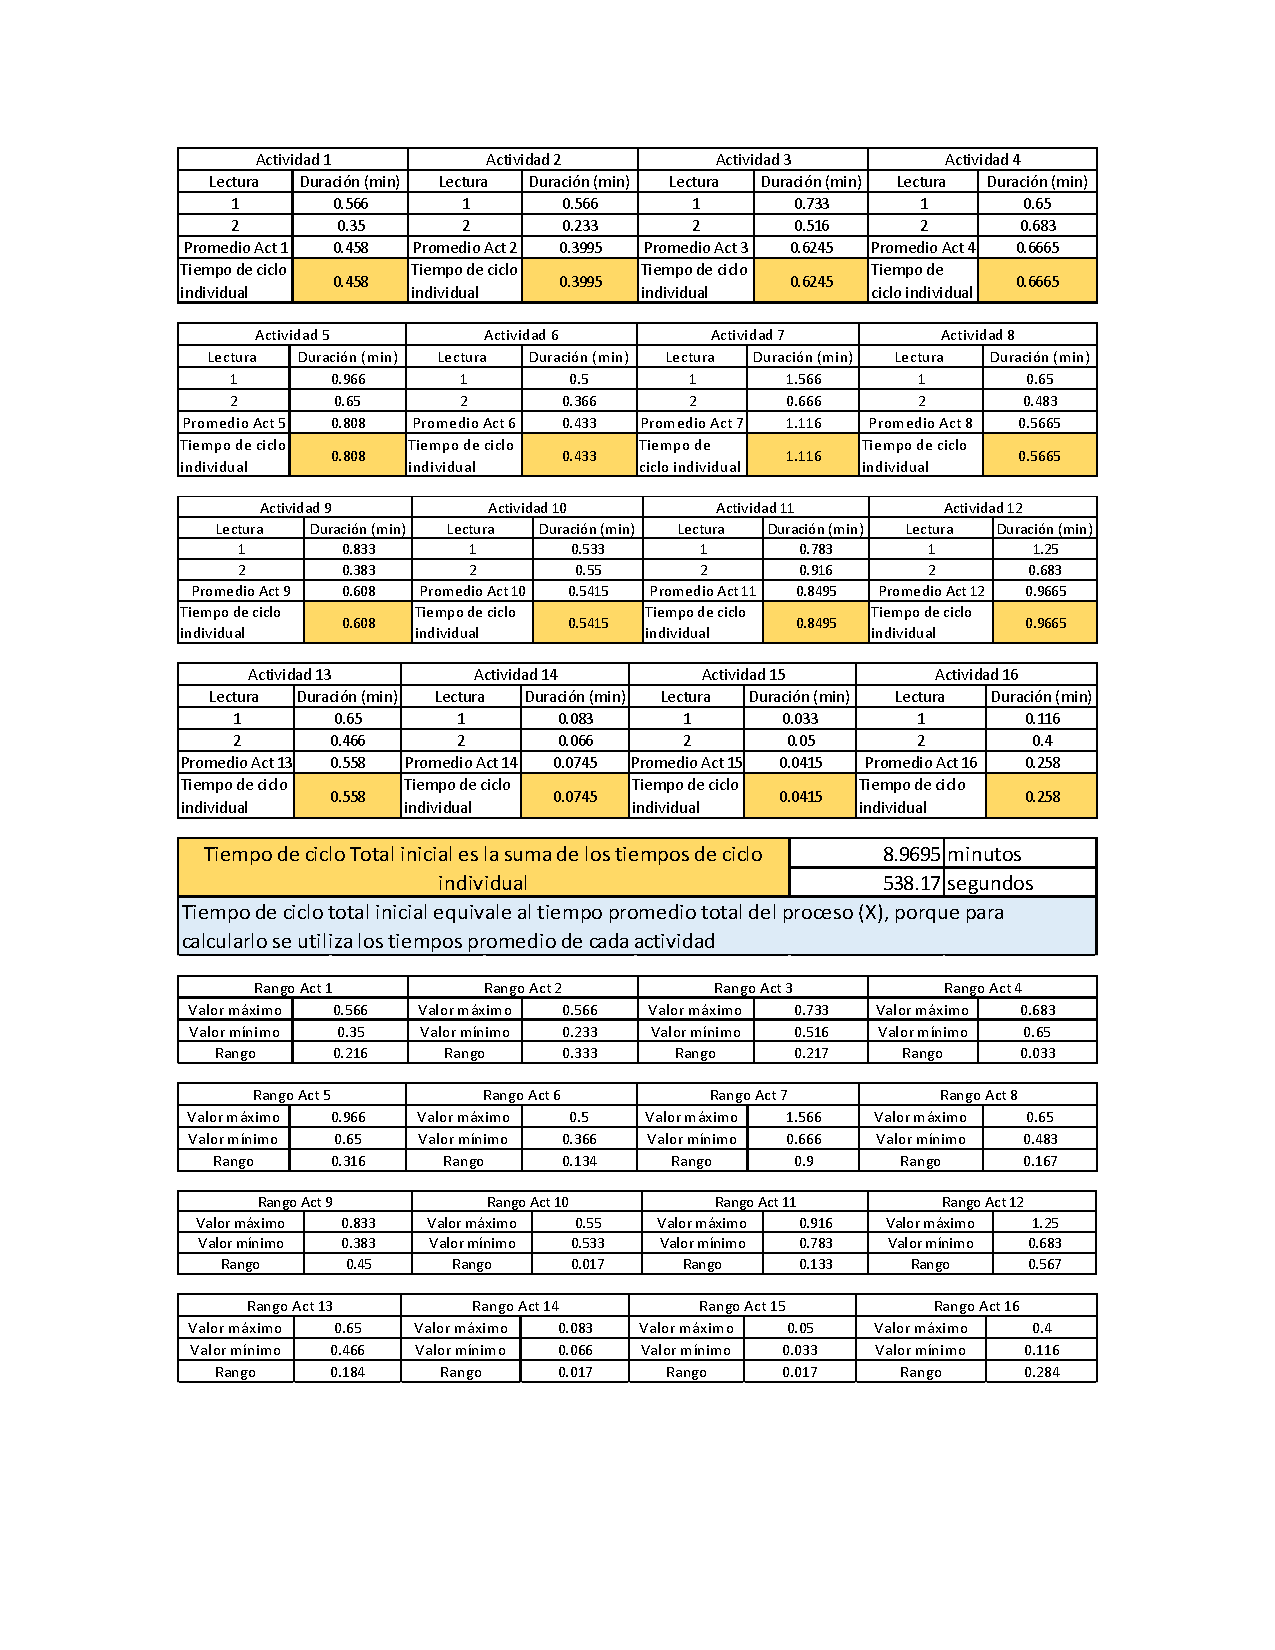
\includepdf[pages=-]{35/Img/tiempoCicloEnsamble.pdf}
    
    Se obtuvo el tiempo ciclo de todas las actividades pero ahora se complemento con muestras de demás compañeros, se utilizo una muestra de 10 lecturas con los siguientes resultados: 
    \newline
    Tiempo de ciclo total: 7.5101 minutos / 450.606 segundos
    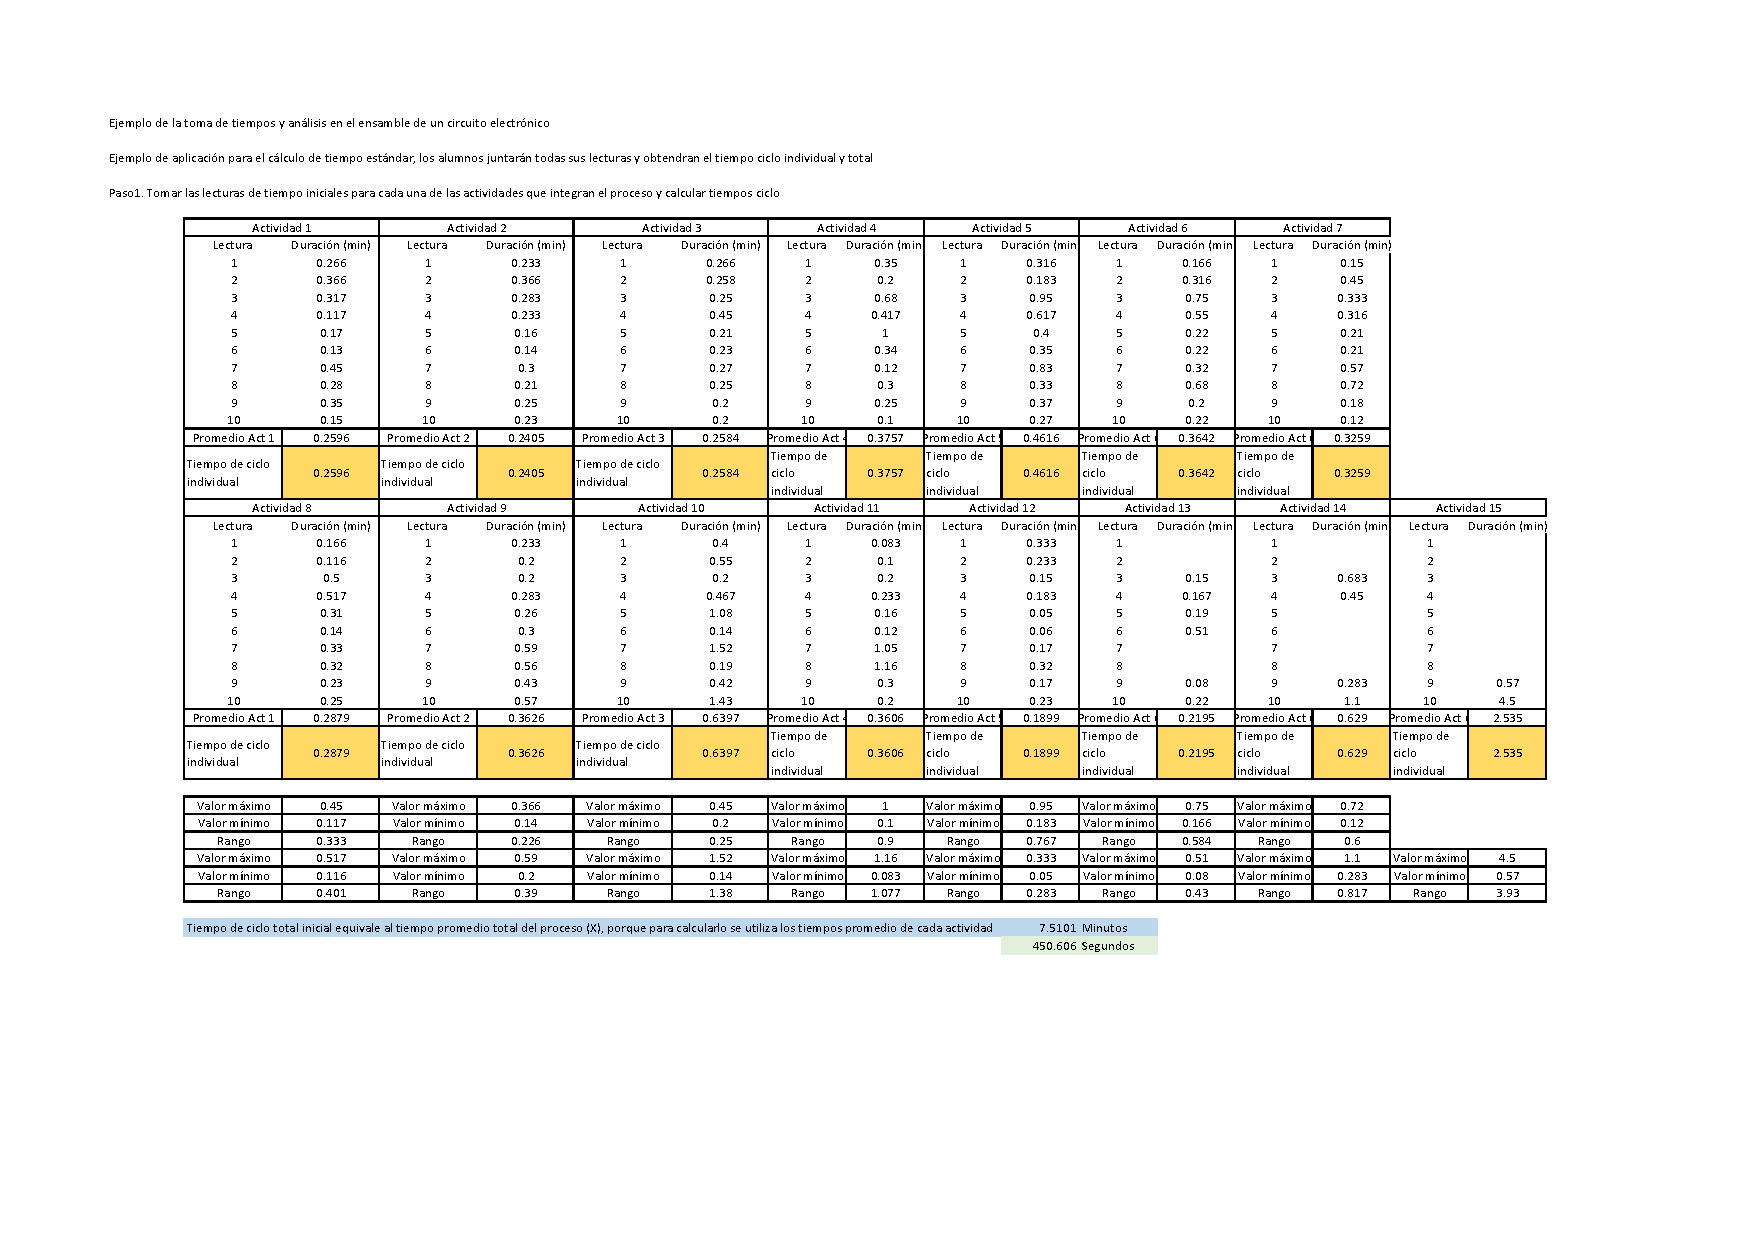
\includepdf[pages=-]{35/Img/tCE10Muestras.pdf}
    
    Una vez obtenido el tiempo ciclo total se puede proceder a obtener el tiempo estándar; para ello tenemos que determinar un factor de desempeño que en este caso lo obtuvimos mediante el sistema whesting house, en este sistema se divide en 4 aptitudes el trabajo y el analista le asigna una calificación de acorde a el trabajo observado y cada calificación tiene una valoración numérica las cuales al final se suman las 4 aptitudes y se les suma 1 para obtener el factor de desempeño. El resultado del sistema whesting house es el siguiente:
    \begin{figure}[H]
        \centering
        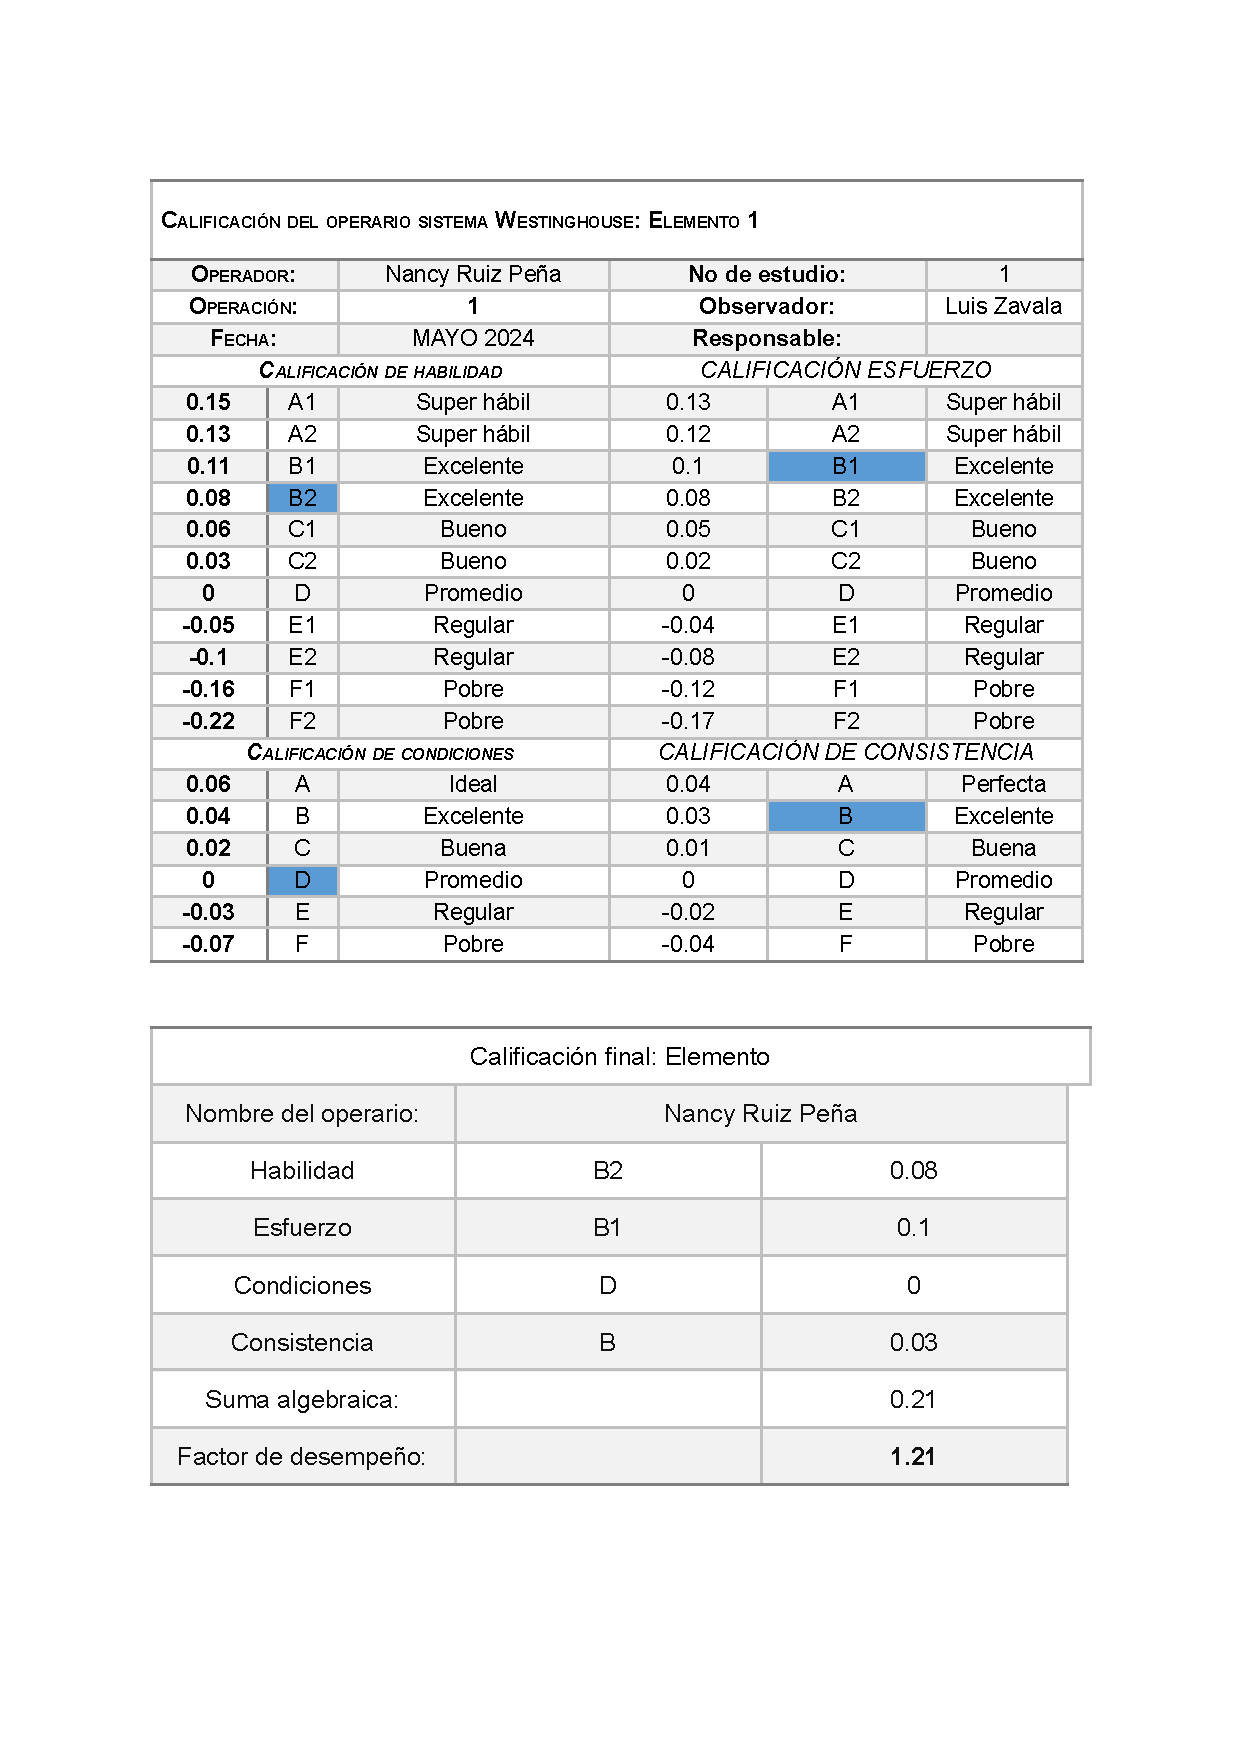
\includegraphics[scale=0.43]{35/Img/sistemaWH.pdf}
        \caption{Sistema WH}
        % \label{WH}
    \end{figure}
    
    El resultado del factor de desempeño nos dio 1.21, finalmente este factor de desempeño lo multplicamos por el tiempo ciclo total y como resultado nos dara el tiempo estandar
    
    \begin{equation}
        TE= (Tiempo Ciclo)(1 + Suma de Valores WH)
    \end{equation}
    
    sustituyendo valores:
    \begin{equation}
        Tiempo Estandar= (3.15)(1.21)=3.81 Minutos
    \end{equation}
    
    \section{Conclusiones}
    
    El proyecto integrador del estudio de movimientos aplicado en un circuito eléctrico se realizo de una manera satisfactoria debido a que se aplicaron los conocimientos adquiridos como lo es el muestreo principalmente, y una vez aplicados estas herramientas se pudo determinar el tiempo estándar del ensamble.
    Los conocimientos adquiridos servirán en la practica en el como desarrollar proyectos desde cero y principalmente el uso de nuevas herramientas tecnológicas como Git Y VisualStuio.
    
    \section{Agradecimientos}
    
    
    \section*{Referencias}
    
    % Ejemplo
    %  @Article{article,
    % 	author = "Author1 LastName1 and Author2 LastName2 and Author3 LastName3",
    % 	title = "Article Title",
    % 	volume = "30",
    % 	number = "30",
    % 	pages = "10127-10134",
    % 	year = "2013",
    % 	doi = "10.3389/fnins.2013.12345",
    % 	URL = "http://www.frontiersin.org/Journal/10.3389/fnins.2013.12345/abstract",
    % 	journal = "Frontiers in Neuroscience"
    % }
    
    % @book{book,
    %   author    = {Author Name}, 
    %   title     = {The title of the work},
    %   publisher = {The name of the publisher},
    %   address   = {The city},
    %   year      = 1993,
    % }
    
    % @incollection{chapter,
    %   author       = {Bauthor Surname}, 
    %   title        = {The title of the work},
    %   editor       = {Editor Name},
    %   booktitle    = {The title of the book},
    %   publisher    = {The name of the publisher},
    %   address      = {The city},
    %   year         = 2002,
    %   pages        = {201-213},
    % }
    
    % @InProceedings{conference,
    %   author = {Cauthor Name and Dauthor Surname and Fauthor LastName},
    %   title = {The title of the work},
    %   booktitle = {The title of the conference proceedings},
    %   year = 1996,
    %   publisher = {The name of the publisher},
    %   editor = {Editor Name1 and Editor Name2},
    %   pages = {41-50},
    % }
    
    % @book{cho,
    %   author       = {Gauthor Name1}, 
    %   title        = {The title of the work},
    %   publisher = {Country code and patent number},
    %   address      = {Patent Country},
    %   year = 2013
    % }
    
    % @book{patent,
    %   author    = {Hauthor Surname1}, 
    %   title     = {The title of the work},
    %   publisher = {Patent number},
    %   address   = {Patent country},
    %   year      = 2010,
    % }
    
    % % please use misc for datasets
    % @misc{dataset, 
    % 	author = "Author1 LastName1 and Author2 LastName2 and Author3 LastName3",
    % 	title = "Data Title",
    % 	year = "2011",
    % 	doi = "10.000/55555",
    % 	URL = "http://www.frontiersin.org/",
    % }
    
    \bibliographystyle{ieeetr}
    \bibliography{35/referencias}
    % 
    % 
    %%%%%%%%%%%%%%%%%%%%%%%%%%%%%%%%%%
    \appendix
    %%%%%%%%%%%%%%%%%%%%%%%%%%%%%%%%%%
    % 
    % 
    \newpage
    
    
    % 
    \centering{\section[\appendixautorefname{}]{Apéndice}}\label{anexo:manual}
    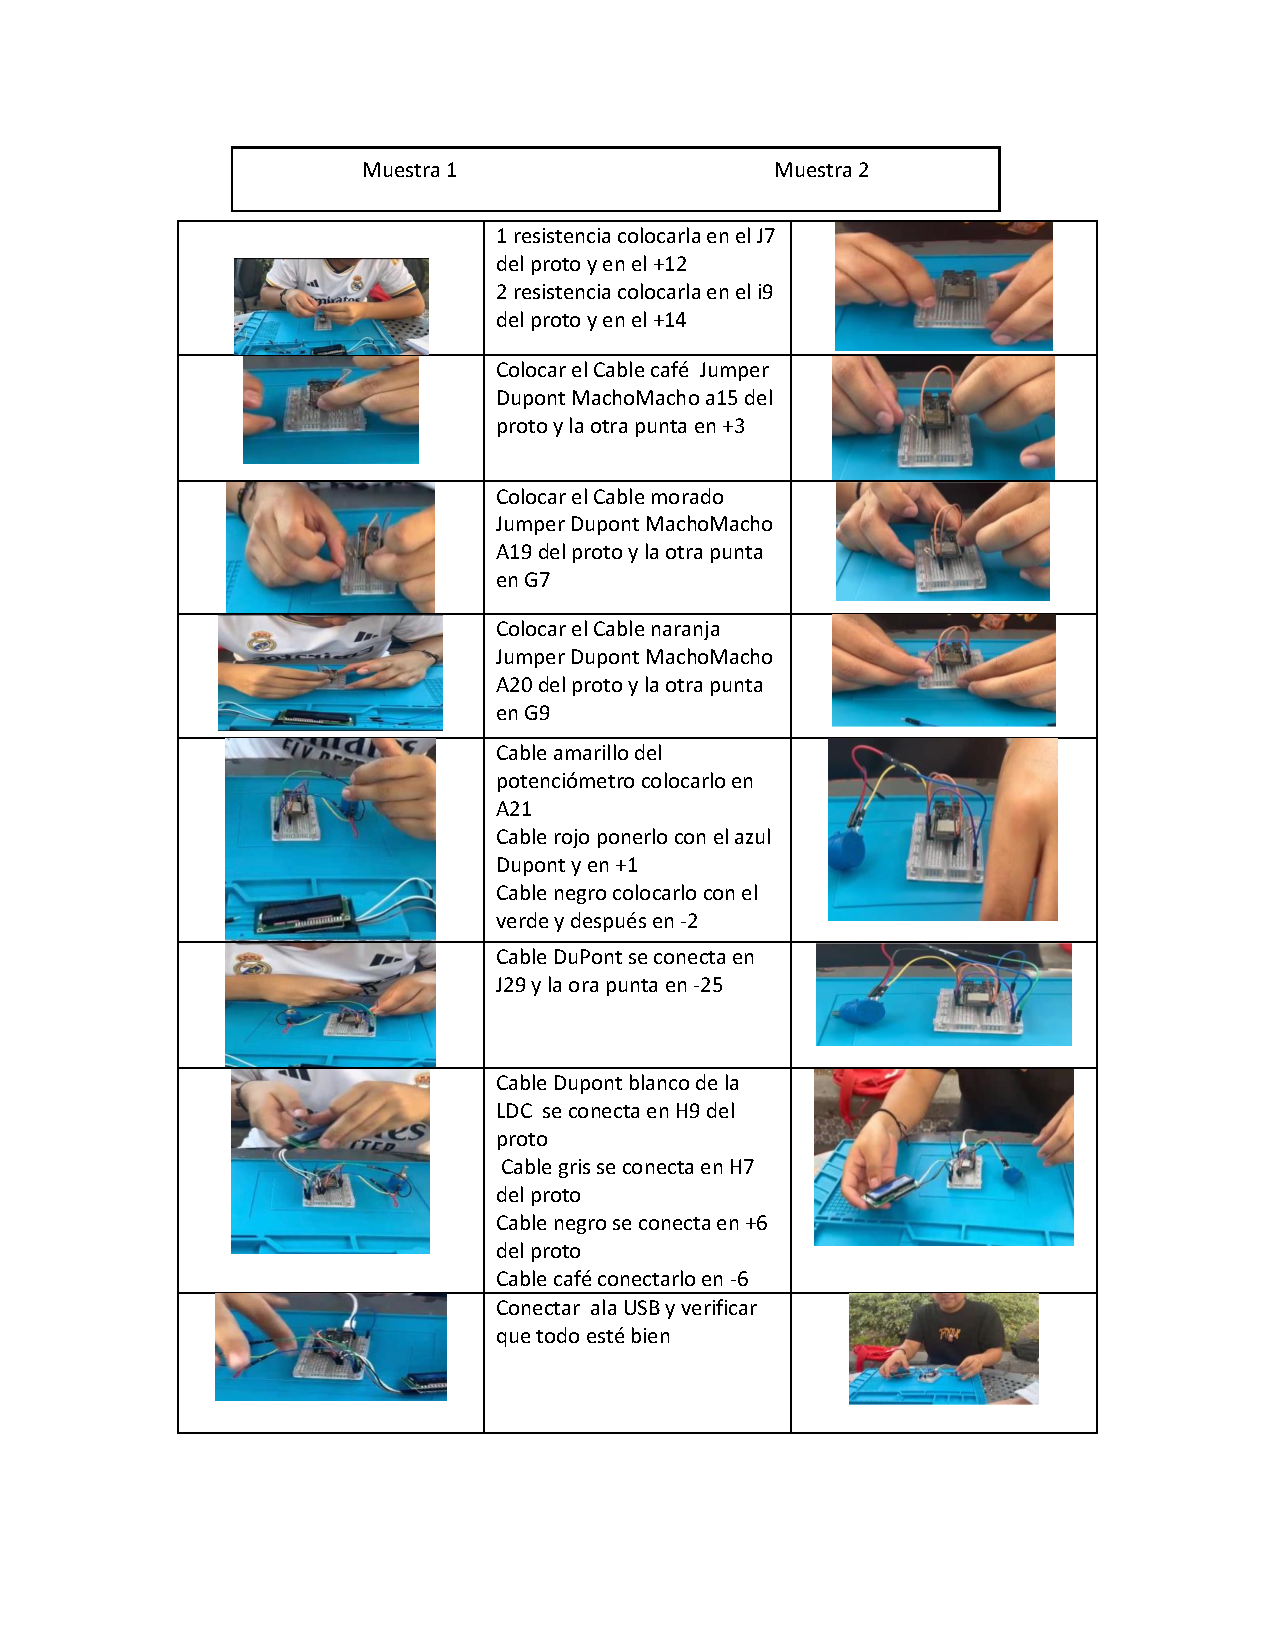
\includepdf[pages=-]{35/Img/manual.pdf}
    %
    
    
    
    
    
    %%%%%%%%%%%%%%%%%%%%%%%%%%%%%%%%%%%%%%%%